%%%%(c)
%%%%(c)  This file is a portion of the source for the textbook
%%%%(c)
%%%%(c)    Abstract Algebra: Theory and Applications
%%%%(c)    Copyright 1997 by Thomas W. Judson
%%%%(c)
%%%%(c)  See the file COPYING.txt for copying conditions
%%%%(c)
%%%%(c)
\chap{Introduction to Rings and Fields}{rings}

\begin{quote}
The integers are like a golden ring in a chain, whose beginning is a glance and whose ending is eternity.     
\emph{(Source:  Khalil Gibran (\emph{paraphrase}))}
\end{quote}

\begin{quote}
The kingdom of heaven is like treasure hidden in a field. When a man found it, he hid it again, and then in his joy went and sold all he had and bought that field.(Source:  Jesus of Nazareth (quoted by Matthew))
\end{quote}

Groups and  \emph{rings} are the two basic abstract structures in study of abstract algebra, These are not the only abstract structures studied,but most others are  modifications of these two. groups and rings are basic in the areas of particle physics, cryptography, and coding theory (see Section~\ref{sec:rings:refs} for more information). They also creep into other areas of mathematics like analysis and number theory.
 As we proceed, you may notice many similarities between the properties of rings and those of groups. Let's begin with a review of common number systems.

This chapter is by Christy Douglass and Chris Thron, with contributions by Jennifer Lazarus and Adam McDonald.

\section{Definitions and Examples \quad\sectionvideohref{xKUyYlAq24c&feature=youtu.be}}
\label{sec:rings:Definitions and Examples}

Some of the number systems we've studied in previouos chapters are:
\begin{itemize}
\item ${\mathbb Z}$=integers
\item ${\mathbb Q}$=rational numbers
\item ${\mathbb R}$=real numbers
\item ${\mathbb C}$=complex numbers
\item ${\mathbb Z}_n$=integers mod n.
\item ${\mathbb Z}[x],  {\mathbb Q}[x], {\mathbb R}[x], \ldots$ = polynomials with coefficients in ${\mathbb Z, \mathbb Q, \mathbb R  \ldots}$     
\end{itemize}

When studying rings (and groups), we put a lot of focus on the integers.  The integers ${\mathbb Z}$ have two operations: addition(+) and multiplication($\cdot$). These operations have the following properties:
\begin{enumerate}[(I)]
\item Closure: if $a, b \in {\mathbb Z}$ then $a+b$ and $a\cdot b$ are in ${\mathbb Z}$.
\item Associativity: if $a, b, c\in {\mathbb Z}$ then $(a+b)+c=a+(b+c)$ and $(a\cdot b)\cdot c=a\cdot (b\cdot c)$.
\item Zero: there is an element $0\in {\mathbb Z}$ such that for all $a\in {\mathbb Z},~a+0=0+a=a$.
\item One: there is an element $1\in {\mathbb Z}$ such that for all $a\in {\mathbb Z},~a\cdot 1=1\cdot a=a$.
\item Commutativity of Addition: if $a,~b\in {\mathbb Z}$, then $a+b=b+a$. 
\item Additive Inverses: for every $a\in {\mathbb Z}$, there exists an element $-a\in {\mathbb Z}$ such that $a+(-a)=0$.
\item Distributivity: for every $a,~b,~c\in {\mathbb Z}$ we have that $a(b+c)=ab+ac$ and $(b+c)a=ba+ca$.\\

\textbf{Note} that commutativity of multiplication is \underline{not} a property of all  rings, so $a(b+c)=(b+c)a$ is not necessarily true for a ring.
 \end{enumerate}

All of the number systems listed at the beginning of this chapter have properties I-VII.  Similar properties are found in other number systems.\footnote{The reader may recall that some of these same properties were listed in Section~\ref{polycoefficients}, when we were talking about coefficients of polynomials.}

\begin{defn}\label{def:ring}
Any number system with the two arithmetic operations (+ and $\cdot$) that satisfy properties I-VII is called a \term{ring}.
\end{defn}

As well as having properties $I-VII$, multiplication is commutative in all of the above number systems. This leads us to the following definition:

\begin{defn}\label{def:comring}
A number system is a \term{commutative ring} if it is a ring where multiplication is also commutative.
\end{defn}

The properties of a ring are so similar to those of a group that it warrants a short discussion. The main difference between a ring and a group is that a ring has two binary operations (usually called addition and multiplication) while a group has only one operation.  In fact, if you consider just the operation of addition, then a ring is a group with respect to addition. As far as multiplication, a ring is ``almost'' a group with respect to multiplication except that not all elements have multiplicative inverses.

Now that we know what a ring is, how do we prove a number system forms a ring? If you said that we would have to prove that the number system fulfills properties $I-VII$, then you would be correct!  Let's look at some examples that will show us how to prove a number system forms a ring.

The rings we've talked about so far (${\mathbb Z},{\mathbb Q},{\mathbb R},{\mathbb C}$) have all been infinite rings. But there are finite rings as well.  In fact ${\mathbb Z}_n$ is also a ring for any integer $n \ge 2$. We'll show this in the following example:

\begin{example}{Zn_ring}
Prove that ${\mathbb Z}_n$ is a ring for any integer $n \ge 2$.

\begin{proof}
Recall that ${\mathbb Z}_n=\{0,1,2,\ldots,n-1\}$.  It is also important to note that the operations of addition and multiplication will be defined as \emph{modular sum} and \emph{modular product}, notated as $\oplus$ and $\odot$, respectively.  We should address each of the seven properties listed above to show that we have a ring.  It turns out that we have already shown each of these properties in the chapter on modular arithmetic, Chapter \ref{modular}.  Let's divide our proof into seven steps, one for each required ring property.
\begin{enumerate}[(I)]
\item First we must show that ${\mathbb Z}_n$ is closed under $\oplus$ and $\odot$.  In Proposition \ref{proposition:modular:closed_property_Zn}, we showed that the modular sum and modular product of two elements of  ${\mathbb Z}_n$ are also in ${\mathbb Z}_n$. In other words, $a\oplus b \in{\mathbb Z}_n$ and $a\odot b\in{\mathbb Z}_n$, for all $a,b\in{\mathbb Z}_n$.  So ${\mathbb Z}_n$ is closed under $\oplus$ and $\odot$.
%%%% Help with reference of the proposition.
\item Second, we must show that the associative property holds for ${\mathbb Z}_n$.  In Proposition \ref{proposition:modular:Zn_comm_assoc} (b), we show that $(a \oplus b) \oplus c  =  a \oplus (b \oplus c)$ and $(a \odot b) \odot c    =  a \odot (b \odot c)$.  So the associative property holds for ${\mathbb Z}_n$.
\item Third, we will show that the zero property holds for ${\mathbb Z}_n$. In Proposition \ref{proposition:modular:id_property_Zn}, we show that $0 \in {\mathbb Z}_n$ and $a\oplus 0=0\oplus a=a$, for any $a\in{\mathbb Z}_n$, so $0$ is the additive identity of ${\mathbb Z}_n$ and the zero property holds.
\item Our next step is to show that ${\mathbb Z}_n$ has the multiplicative identity property (one).  Again, we will refer to Section \ref{ArithWithRems}.  In particular, Exercise \ref{exercise:modular:56} showed us that $1\in{\mathbb Z}_n$ and $1\odot a=a\odot 1=a$, for any $a\in{\mathbb Z}_n$.  So, the identity property of multiplication holds for ${\mathbb Z}_n$.
\item The commutative property of $\oplus$ for ${\mathbb Z}_n$ must be proven next.  Proposition \ref{proposition:modular:Zn_comm_assoc} (a) shows us that $a \oplus b   =  b \oplus a$ and
$a \odot b    =  b \odot a$, for all $a,b\in{\mathbb Z}_n$.  Note that for a set to be a ring, we only need to show that commutativity of \emph{addition} holds.  Because commutativity of \emph{multiplication} also holds for ${\mathbb Z}_n$, we may also have a \emph{commutative} ring.  Let's continue with our proof that ${\mathbb Z}_n$ is a ring before we jump to that conclusion.
\item The sixth property that we must show is that of the additive inverse.  We will refer back to Proposition \ref{proposition:modular:addinv_property_Zn}.  Here we let $a' = n-a$, for any $a\in{\mathbb Z}_n$.  We show that $a'\in{\mathbb Z}_n$ and $a \oplus a' = a' \oplus a  = 0 \pmod{ n}$: that is, $a'$ is the additive inverse of $a$.
\item For our last step, we will show that the distributive property holds true for ${\mathbb Z}_n$. Once again, we have already shown that this is true.  In Proposition \ref{proposition:modular:Zn_comm_assoc} (c), we show that $a \odot (b \oplus c)  = (a \odot b)\oplus (a \odot c)$.  Since $\odot$ commutes in ${\mathbb Z}_n$, it follows that $a \odot (b \oplus c)  = (b \oplus c) \odot a= (a \odot b)\oplus (a \odot c)$ and the distributive property holds.
\end{enumerate}
We have shown that all seven ring properties hold true in ${\mathbb Z}_n$ over $\oplus$ and $\odot$. Additionally, we have shown that ${\mathbb Z}_n$ commutes over $\odot$.  So, ${\mathbb Z}_n$ is a \emph{commutative} ring and our proof is complete.
\end{proof}
\end{example}

We've already mentioned that ${\mathbb Q}$ is a ring. Sometimes we can use rings to create larger rings by adding additional elements. Such rings are called \term{extension rings}. We will discuss these further in Section~\ref{sec:extensionRings}. For now, let's look at a particular example.

\begin{example}{extension_ring}
Prove that ${\mathbb Q}[\sqrt[3]{2}]=\{a_0+a_1\sqrt[3]{2}+a_2(\sqrt[3]{4})~|~a_0,a_1,a_2\in {\mathbb Q}\}$ forms a ring.\\

\underline{Note}: ${\mathbb Q}[\sqrt[3]{2}]$ is the set of all polynomials of the form:

$a_0(\sqrt[3]{2})^0+a_1(\sqrt[3]{2})^1+a_2(\sqrt[3]{2})^2+\cdots+a_n(\sqrt[3]{2})^n$, where $a_0,a_1,a_2,\cdots,a_n\in~{\mathbb Q}$.\\

In this case, we have defined ${\mathbb Q}[\sqrt[3]{2}]$ using only the first three terms.\\ 
(We will explain why three terms is enough later on in the proof.) \\

\begin{proof}
To prove that ${\mathbb Q}[\sqrt[3]{2}]$ forms a ring, we must show ${\mathbb Q}[\sqrt[3]{2}]$ has all seven ring properties listed above. It will be useful to define a couple of arbitrary elements in our set:
let $a,b\in{\mathbb Q}[\sqrt[3]{2}]$ such that:
$a=a_0+a_1\sqrt[3]{2}+a_2\sqrt[3]{4}$ and $b=b_0+b_1\sqrt[3]{2}+b_2\sqrt[3]{4}$.
\medskip

Property (1):  First, we need to prove that ${\mathbb Q}[\sqrt[3]{2}]$ is closed under addition and multiplication. We will divide this task into two parts:
\begin{enumerate}[(a)]

\item If $a,b\in{\mathbb Q}[\sqrt[3]{2}]$ then $a+b\in {\mathbb Q}[\sqrt[3]{2}]$. This is called \emph{additive closure}.
\item If $a,b\in{\mathbb Q}[\sqrt[3]{2}]$ then $ab\in {\mathbb Q}[\sqrt[3]{2}]$. This is called \emph{multiplicative closure}.
\end{enumerate}
First, we will look at additive closure (a).

Remember that we have already defined two arbitrary elements in ${\mathbb Q}[\sqrt[3]{2}]$, $a$ and $b$. So,
\begin{align*}
a+b&=(a_0+a_1\sqrt[3]{2}+a_2\sqrt[3]{4})+(b_0+b_1\sqrt[3]{2}+b_2\sqrt[3]{4})\\
&=(a_0+b_0)+(a_1+b_1)\sqrt[3]{2}+(a_2+b_2)\sqrt[3]{4}.
\end{align*}
Now let $c_0=(a_0+b_0)$, $c_1=(a_1+b_1)$ and $c_2=(a_2+b_2)$. Since ${\mathbb Q}$ is closed under addition, then $c_0,c_1,c_2\in{\mathbb Q}$ and $a+b=c_0+c_1\sqrt[3]{2}+c_2\sqrt[3]{4}.$ It should now be clear that this sum is indeed an element of $\in{\mathbb Q}[\sqrt[3]{2}]$. We have shown that adding any two elements in ${\mathbb Q}[\sqrt[3]{2}]$ will always produce another element of ${\mathbb Q}[\sqrt[3]{2}]$. So, ${\mathbb Q}[\sqrt[3]{2}]$ is closed under addition.

Now let's prove multiplicative closure $(b)$.
We will again use $a$ and $b$ as defined earlier, so that: 
\begin{align*}
ab&=(a_0+a_1\sqrt[3]{2}+a_2\sqrt[3]{4})(b_0+b_1\sqrt[3]{2}+b_2\sqrt[3]{4})\\ &=(a_0b_0+2a_1b_2+2a_2b_1)+(a_0b_1+a_1b_0+2a_2b_2)\sqrt[3]{2}\\
& +(a_0b_2+a_1b_1+a_2b_0)\sqrt[3]{4}.
\end{align*}
Again, we must show that this product is also an element of ${\mathbb Q}[\sqrt[3]{2}]$.  Let's use a strategy similar to the one we used for additive closure.

Suppose we let $d_0,d_1,d_2\in{\mathbb Q}$ such that $d_0=(a_0b_0+2a_1b_2+2a_2b_1)$, $d_1=(a_0b_1+a_1b_0+2a_2b_2)$, and $d_2=(a_0b_2+a_1b_1+a_2b_0)$.  Since ${\mathbb Q}$ is closed under multiplication, then $d_0,d_1,d_2\in{\mathbb Q}$ and $ab=d_0+d_1\sqrt[3]{2}+d_2\sqrt[3]{4}\in{\mathbb Q}[\sqrt[3]{2}]$. We have shown that multiplying any two elements in ${\mathbb Q}[\sqrt[3]{2}]$ produces another element in ${\mathbb Q}[\sqrt[3]{2}]$, so ${\mathbb Q}[\sqrt[3]{2}]$ is closed under multiplication.\\

\begin{exercise}{threeTermsofQring}
Recall that in our definition of ${\mathbb Q}[\sqrt[3]{2}]$, we only included three terms in the polynomial expansion. In this exercise, we will see why. 
\begin{enumerate}[(a)]
\item Show that if we include 4 terms, then we get the same set. In other words, show that any polynomial of the form $d_0+d_1\sqrt[3]{2}+d_2\sqrt[3]{4}+d_3(\sqrt[3]{2})^3$ can also be rewritten in the form $a_0+a_1\sqrt[3]{2}+a_2\sqrt[3]{4}$ where $a_0, a_1, a_2  \in {\mathbb Q}$.
\item
Show similarly that if we include 5 terms, we still get the same set (use a similar method).
\item
Given a polynomial of the form $d_0+d_1\sqrt[3]{2}+d_2\sqrt[3]{4}+ \ldots + d_n(\sqrt[3]{2})^n$, show that it can be rewritten in the form $a_0+a_1\sqrt[3]{2}+a_2\sqrt[3]{4}$ where $a_0, a_1, a_2  \in {\mathbb Q}$ by giving explicit formulas for $a_0, a_1, a_2$.
\item
In the definition of ${\mathbb Q}[\sqrt[3]{2}]$, we included a term proportional to $\sqrt[3]{4}$.  Show that this term is necessary, by showing that $a_0+a_1\sqrt[3]{2}$ is \emph{not} closed under multiplication.
\end{enumerate}
\end{exercise}

Let's continue with our proof of Example \ref{example:rings:extension_ring}. We have shown that ${\mathbb Q}[\sqrt[3]{2}]$ satisfies the first property of rings. Now, let's take a look at property (2). We must show associativity for addition and multiplication. In other words, we must show that:
\begin{enumerate}[(a)]
\item If $a,b,c\in{\mathbb Q}[\sqrt[3]{2}]$ then $(a+b)+c=a+(b+c)$, and
\item If $a,b,c\in{\mathbb Q}[\sqrt[3]{2}]$ then $(ab)c=a(bc)$.
\end{enumerate}

For associativity of addition, let $a,b,c,\in{\mathbb Q}[ \sqrt[3]{2}]$. Since all of the numbers in ${\mathbb Q}[\sqrt[3]{2}]$ are real numbers, and the real numbers are associative, then it follows automatically that numbers in ${\mathbb Q}[\sqrt[3]{2}]$ also associate.  We can make a similar argument for associativity of multiplication.  Associativity is an example of an \emph{inherited property}.

\begin{defn}\label{def:inherited property}
An \term{inherited property} is a property such that, if the property is true for a set of numbers $S$, then it's also true for any subset of $S$.
\end{defn}

\begin{exercise}{addClosureNotInherited}
Show that additive closure is \emph{not} an inherited property by providing a counterexample.
\end{exercise}{}

Back to our proof of Example \ref{example:rings:extension_ring}.

Property (3): This is known as the \emph{zero property}. To prove this property, we must show that $0\in{\mathbb Q}[\sqrt[3]{2}]$ and also that $a+0=0+a=0$ for all $a\in{\mathbb Q}[\sqrt[3]{2}]$. Notice that $0=0+0\sqrt[3]{2}+0\sqrt[3]{4}\in{\mathbb Q}[\sqrt[3]{2}]$. Since all numbers, $a\in{\mathbb Q}[\sqrt[3]{2}]$ are real numbers, it follows that $a+0=0+a=0$. So $0$ is the zero element of ${\mathbb Q}[\sqrt[3]{2}]$ and property (3) holds true.\\

The proof of property (4) is left as an exercise.

\begin{exercise}{identityQcuberoot2}
Prove that 1 is the identity of ${\mathbb Q}[\sqrt[3]{2}]$. (You may use the proof of the zero element as a model.)  
\end{exercise}{}

The proofs of properties (5) and (7) resemble the proof of property (2).

\begin{exercise}{comm/distPropsQcuberoot2}
Prove properties (5) and (7). (You may use the proof of property (2) as a model.)
\end{exercise}{}

We have shown that ${\mathbb Q}[\sqrt[3]{2}]$ satisfies all seven properties of rings. Therefore, by Definition \ref{def:ring}, ${\mathbb Q}[\sqrt[3]{2}]$ is a ring and our proof is complete.
\end{proof}
\end{example}{}

\begin{exercise}{Qsqrt2ring}
Let ${\mathbb Q}[2^{\frac{1}{2}}]$ be the set of all numbers $\{a+b\cdot2^{\frac{1}{2}}\}$ with $a,b\in {\mathbb Q}$. Is ${\mathbb Q}[2^{\frac{1}{2}}]$ a ring?
\end{exercise}

\begin{exercise}{ringMatrices}
\begin{enumerate}[(a)]
\item Let ${\mathbb M}_2({\mathbb R})$ be the set of  $2\times 2$ matrices with entries in ${\mathbb R}$. Show that ${\mathbb M}_2({\mathbb R})$ is a ring under the operations of matrix addition and multiplication.
\item Give an example to show that ${\mathbb M}_2({\mathbb R})$ is not commutative under multiplication.
\item Show that although the distributive law holds in ${\mathbb M}_2({\mathbb R})$, it is \emph{not} true that $X(Y+ Z) = YX + ZX$ for all $a,b,c \in {\mathbb M}_2({\mathbb R})$. This shows that you have to be very careful about the order of multiplication when dealing with rings that aren't commutative.
\end{enumerate}
\end{exercise}{}

\begin{exercise}{circulant_matrices}
Define the set $C_3({\mathbb R})$ as the set of all $3\times3$ \term{circulant matrices} of the form:
$\begin{bmatrix}
a & c & b\\
b & a & c\\
c & b & a\\
\end{bmatrix}$,
where $a,b,c\in{\mathbb R}$.  Prove or disprove that $C_3({\mathbb R})$ is a ring.
\end{exercise}

\begin{exercise}{}
Suppose $R$ is a ring. Prove that  ${\mathbb M}_2(R)$ is also a ring.
\end{exercise}


\subsection{Polynomial  rings}\label{sec:polynomialRings}

Take any ring $R$ and the set of polynomials over that ring $R[x]$.  It turns out that $R[x]$ is also a ring.  In this section, we will prove this, and explore some properties of $R[x]$. 

Actually, we've already completed most of the proof that $R[x]$ is a ring. Recall that in Section~\ref{polycoefficients} we proved several properties of polynomials $R[x]$, under very general assumptions about the set of coefficients $R$.  In fact, properties (I)-(V) in Section~\ref{polycoefficients} are all included in the ring properties listed in Section~\ref{sec:rings:Definitions and Examples}. So all of the properties shown in Section~\ref{polycoefficients} apply to $R[x]$ as long as $R$ is a ring.

\begin{exercise}{polyRingProps}
Go back to Section~\ref{polycoefficients} and identify the propositions that prove that the set $R[x]$ satisfies the ring properties (I,II,III,V,VI,VII) from Section~\ref{sec:rings:Definitions and Examples}.
\end{exercise}

We are still missing property IV, the identity property. We can take care of this in short order.

\begin{exercise}{}
Show that the polynomial $p(x) = 1x^0$ is a multiplicative identity for the set of polynomials $\mathbb{C}[x]$.
\end{exercise}

\begin{prop}{ringMultId}
Suppose that $R$ is a ring with a multiplicative identity 1. Then $1x^0$ is a multiplicative identity of $R[x]$.
\end{prop}

\begin{exercise}{}
Prove Proposition~\ref{proposition:rings:ringMultId}.
\end{exercise}

Putting Exercise~\ref{exercise:rings:polyRingProps} and Proposition \ref{proposition:rings:ringMultId} together, we have immediately:

\begin{prop}{polyringsarerings} The set of polynomials over a ring is also a ring. That is, if $R$ is a ring, then $R[x]$ is also a ring.
\end{prop}

Proposition~\ref{proposition:rings:polyringsarerings} is a powerful result. We may use this proposition to build larger and larger rings. For example, Proposition~\ref{proposition:rings:polyringsarerings} tells us that $((\mathbb{Z}[x])[y])[z]$ is a ring of polynomials in $x,y,z$  (usually this is written as $\mathbb{Z}[x,y,z]$). Apparently there are many examples of mathematical structures that are rings, which makes them an interesting and fruitful object of study.



\subsection{Some Ring Proofs}

Remember that rings must satisfy the multiplicative identity property. For the set of integers, the multiplicative identity is uniquely 1. We can show that the multiplicative identity for any ring is unique.

\begin{prop}{mult_idR}
The multiplicative identity of a ring, $R$, is unique.\\

\begin{proof}
We need to show that if $x$ is a multiplicative identity, then $x=1$.
\begin{align*}
&\text{x is a multiplicative identity} & \text{Given}\\
&x\cdot1=1\cdot x=1 & \text{Definition of Multiplicative Identity}\\
&\text{1 is a multiplicative identity} & \text{Given}\\  
&1\cdot x=x\cdot1=x & \text{Definition of Multiplicative Identity} \\
&x=1 & \text{Substitution}
\end{align*}
\end{proof}
\end{prop}

\begin{exercise}{addIdenUnique}
Show that the additive identity of a ring $R$ is unique.  (You may model your proof on the proof of Proposition~\ref{proposition:rings:mult_idR}).
\end{exercise}

Way back in Section~\ref{OpsAndRels} we mentioned the \term{zero divisor property} for real numbers: the product of two real numbers is zero if and only if at least one of the two numbers is zero. In fact, the ``only if'' part of this statement is \emph{not true} for general rings:

\begin{exercise}{ModZeroProducts}
\begin{enumerate}[(a)]
\item Show that two nonzero numbers can multiply to give zero in ${\mathbb Z}_6$.
\item Show that if $n$ is not prime, then there are two nonzero numbers in ${\mathbb Z}_n$ that multiply to give zero.
\end{enumerate}
\end{exercise}
We can, however, show the ``if'' part:

\begin{prop}{add_inverse}
Given a ring, $R$, for any $x\in R$ we have $x\cdot0=0\cdot x=0$.

\begin{proof}
We will use properties of rings in our proof.

\begin{align*}
&0=0+0 & \text{Definiton of Additive Identity}\\
&x\cdot0=x\cdot(0+0) & \text{Substitution}\\
&x\cdot0=x\cdot0+x\cdot0 & \text{Distributive Property}\\
&x\cdot0+-(x\cdot0)=(x\cdot0+x\cdot0)+-(x\cdot0) & \text{Substitution}\\
&x\cdot0+-(x\cdot0)=x\cdot0+(x\cdot0+-(x\cdot0)) & \text{Associativity of Addition}\\
&0=x\cdot0+(0) & \text{Additive Inverse}\\
&0=x\cdot0 & \text{Additive Identity}
\end{align*}

We have shown that $0=x\cdot0$. It remains to show that $0=0\cdot x$, since multiplication in rings is not always commutative.

\begin{exercise}{MultZeroRing}
Complete the proof of Proposition \ref{proposition:rings:add_inverse} by showing that $0=0\cdot x$, for $x\in R$.
\end{exercise}
\end{proof}
\end{prop}
In the following proposition, we show that we may construct the additive inverse of any ring element by multiplying the element by the additive inverse of 1.

\begin{prop}{inverse}
Let $R$ be a ring, let $-1$ be the additive inverse of $1$, and let $-x$ denote the additive inverse of $x\in R$. Then $-x=(-1)\cdot x$.
\end{prop}

\begin{exercise}{}
Prove Proposition \ref{proposition:rings:inverse}.
\end{exercise}

Since there are many rules that ring operations obey,
we can simplify algebraic expressions in rings in much the same way as we do in basic algebra.

\begin{exercise}{comm_ring}
Given $A,B,C\in R$ where R is a commutative ring, we can show that $(B+(-C))\cdot(A\cdot(B+C))=A\cdot(B\cdot B+(-C)\cdot C))$. Give the reasons for the following steps in the simplification:
\begin{align*}
(B+(-C))\cdot(A\cdot(B+C))&=(A\cdot(B+C))\cdot(B+(-C)) & \text{Comm. prop.}\\   
&=A\cdot((B+C)\cdot(B+(-C))) & \text{Assoc. prop.}\\
&=A\cdot(((B+C)\cdot B)+((B+C)\cdot(-C))) & \underline{<~1~>}\\
&=A\cdot((B\cdot B+C\cdot B)+(B\cdot (-C)+C\cdot (-C))) & \underline{<~2~>}\\
&=A\cdot((B\cdot B+B\cdot C)+((-C)\cdot(B)+(-C)\cdot C))  & \underline{<~3~>}\\
&=A\cdot(B\cdot B+(B\cdot C+(-C)\cdot(B)+(-C)\cdot C))  & \underline{<~4~>}\\
&=A\cdot(B\cdot B+(B\cdot C+B\cdot(-C))+(-C)\cdot C)) & \underline{<~5~>}\\
&=A\cdot(B\cdot B+(B\cdot(C+(-C))+(-C)\cdot C)) & \underline{<~6~>}\\
&=A\cdot(B\cdot B+(B\cdot(0)+(-C)\cdot C)) & \underline{<~7~>}\\
&=A\cdot(B\cdot B+(0+(-C)\cdot C)) & \underline{<~8~>}\\
&=A\cdot(B\cdot B+(-C)\cdot C)) & \underline{<~9~>}
\end{align*}
\end{exercise}

\section{Subrings}
\label{sec:Subrings}

Earlier we mentioned that two important topics studied in Abstract Algebra are groups and rings. Just like groups have subgroups, rings have \emph{subrings}.

\begin{defn}\label{subring}
A ring that is a subset of another ring is called a \term{subring}.
\end{defn}

Suppose $R$ is a ring, and $S\subset R$. To prove $S$ is a subring, we must show that $S$ satisfies all seven ring properties. $S$ will inherit certain properties (associativity, commutativity, and distributive) from $R$, making lighter work of our proof that $S$ is also a ring. 

To show that $S\subset R$ is a ring, we must show the following:

\begin{itemize}
\item Additive Inverse:  $a\in S\implies-a\in S$.
\item Closure:  $a,b\in S\implies~a+b\in S$ and $ab\in S$.
\item Zero: $0\in S$, such that $0+a=a+0=a$, for all $a\in S$.
\item One:  $1\in S$, such that $1\cdot a=a\cdot 1=a$, for all $a\in S$. Note that for $S$ to be a subring of $R$, the multiplicative identities must be the \underline{same}.
\end{itemize}

If $S$ is a subring of $R$ \emph{except} that $1\notin S$, then $S$ is a \term*{subring} of $R$ \term*{without unity}\index{Subring!Without unity}.\\

Examples of subrings:
\begin{enumerate}[(a)]
\item ${\mathbb Z}$ is a subring in ${\mathbb Q}$.
\item ${\mathbb R}$ is a subring of ${\mathbb C}$.
\item If $R$ is a ring, then $R$ is a subring of $R[x]$.
\end{enumerate}

Let's look at a subring proof together:

\begin{example}{}
Given two rings $R_1$ and $R_2$ which share the same + and $\cdot$ operations, show that $R_1 \cap R_2$ is a subring of both $R_1$ and $R_2$.

\begin{proof}
Let's begin by showing that $R_1 \cap R_2\subset R_1$ and $R_2$.  By definition of $\cap, ~a\in R_1\cap R_2\implies a\in R_1$ and $a\in R_2$. So  $R_1 \cap R_2\subset R_1$ and $R_2$. 

Next, we will show the additive inverse property. Let $a$ be an arbitrary element in $R_1 \cap R_2$. Then $a\in R_1$ and $R_2$, by the definition of $\cap$. Remember that $R_1$ and $R_2$ are rings with the same + operation, so $-a\in R_1$ and $R_2$.  This means that $-a\in R_1 \cap R_2$ and the additive inverse property holds.

Our next task is to show that $R_1 \cap R_2$ contains the zero element. Since $R_1$ and $R_2$ are rings with the same + operation, then $0\in R_1$ and $R_2$.  By definition of $\cap, ~0\in R_1 \cap R_2$, and the zero property holds.

In the following exercise, you will complete the proof that $R_1\cap R_2$ is a subring by showing that it has a multiplicative identity.

\begin{exercise}{}
Given rings $R_1$ and $R_2$, with the same $\cdot$ operation, Show that $1\in R_1 \cap R_2$. You can model your proof after the zero property proof.
\end{exercise}
\end{proof}
\end{example}
We have shown in Exercise~\ref{exercise:rings:ringMatrices} that ${\mathbb M}_2({\mathbb R})$, forms a ring.  In the following exercise, we will consider some subrings of ${\mathbb M}_2({\mathbb R})$.


\begin{exercise}{}
\begin{enumerate}[(a)]
\item
Show that the set of all matrices of the form:
$$
\begin{bmatrix}
a & 0\\
0 & 0
\end{bmatrix}
$$
is a subring of all 2x2 matrices, ${\mathbb M}_2({\mathbb R})$.
\item
Show that the set of all matrices of the form:
$$
\begin{bmatrix}
a & 0\\
0 & b
\end{bmatrix}
$$
is a subring of ${\mathbb M}_2({\mathbb R})$.
\item
Prove or disprove: The set of all matrices of the form:
$$
\begin{bmatrix}
a & 0\\
b & d
\end{bmatrix}
$$
is a subring of  ${\mathbb M}_2({\mathbb R})$.
\end{enumerate}
\end{exercise}

In Section \ref{sec:rings:Definitions and Examples}, we learned that ${\mathbb C}$, the set of all complex numbers, forms a ring.  Consider the following subset of ${\mathbb C}$:

\begin{exercise}{}
Prove or disprove:  $\{1,-1,i,-i\}$ forms a subring of ${\mathbb C}$.
\end{exercise}

\begin{exercise}{}
Let ${\mathbb Z}+{\mathbb Z}i$ denote the set of complex numbers with real and imaginary parts that are both integers. Prove or disprove ${\mathbb Z}+{\mathbb Z}i$ is a subring of ${\mathbb C}$.
\end{exercise}

The set $n{\mathbb Z}$ represents the set of all integers, $n\cdot k\in{\mathbb Z}$, such that $n$ is some integer and $k\in{\mathbb Z}$.  For example, $2{\mathbb Z}$ represents the set of all even integers.  It should be clear that $n{\mathbb Z}\subset{\mathbb Z}$, for all $n\in{\mathbb N}$, but is it a subring as well?

\begin{exercise}{}
\begin{enumerate}[(a)]
\item Prove or disprove: $2{\mathbb Z}$ is a subring (with or without unity)  of ${\mathbb Z}$.
\item Prove or disprove: $3{\mathbb Z}$ is a subring (with or without unity)  of ${\mathbb Z}$.
\item Show that $m{\mathbb Z}$ is a subring (without unity) of $n{\mathbb Z}$ iff n divides m.
\end{enumerate}
\end{exercise}

If $R$ is a finite ring, the addition and multiplication Cayley tables for $S$ can be obtained from the corresponding tables of $R$. We can cross out the rows and columns with heading elements in $R$ that are \emph{not} also in $S$. Let's look at an example.

\begin{example}{}
$\{0,2,4\}$ is a subring of ${\mathbb Z}_6$ without unity.\\

\begin{proof}
The Cayley tables for modular addition and modular multiplication of ${\mathbb Z}_6$ are:\\

\begin{figure}[H]
	   \center{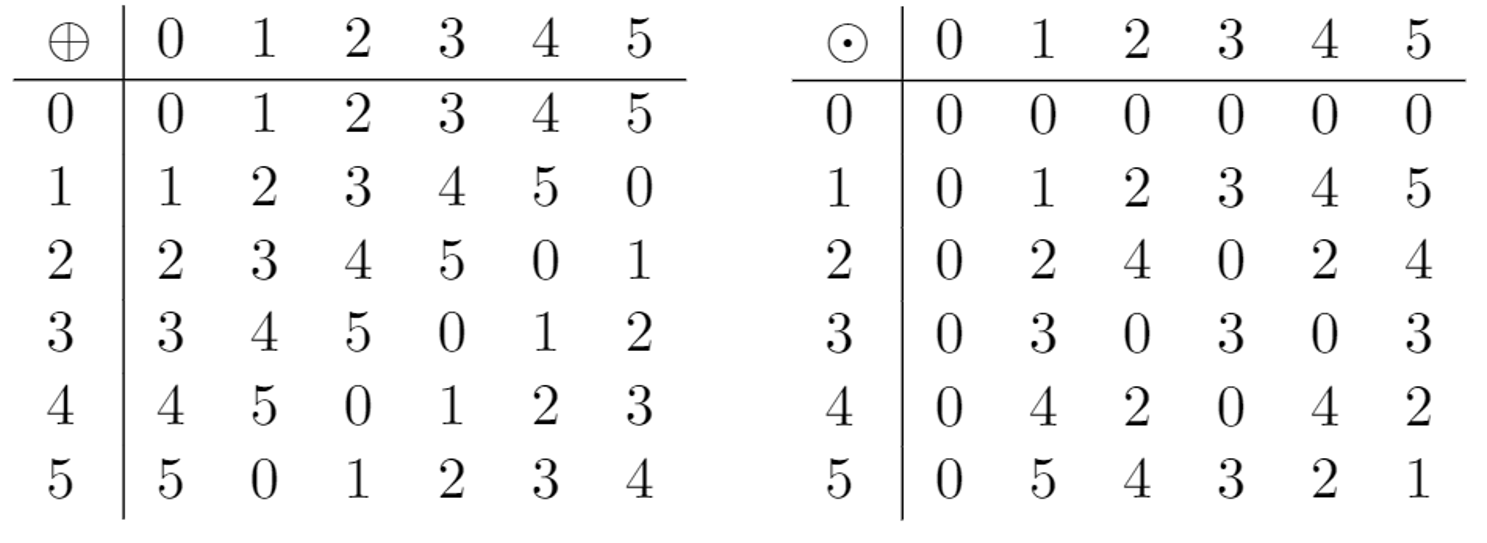
\includegraphics[width=3.5in]
	         {images/origTables.png}}
\end{figure}

Now, we are wanting only $\{0,2,4\}$ of ${\mathbb Z}_6$. We will keep those values and cross out all rows and columns that are not $\{0,2,4\}$. \\

\begin{figure}[H]
	   \center{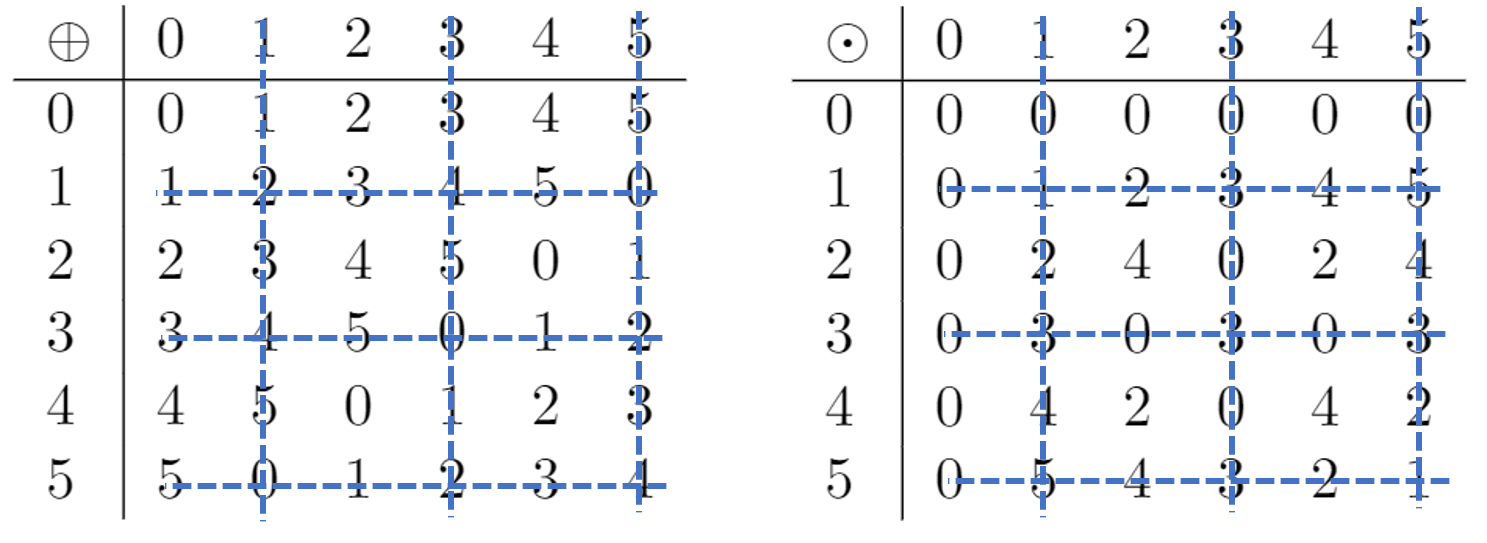
\includegraphics[width=3.5in]
	         {images/crossOutTables.png}}
\end{figure}

This results in the following:

\begin{figure}[H]
	   \center{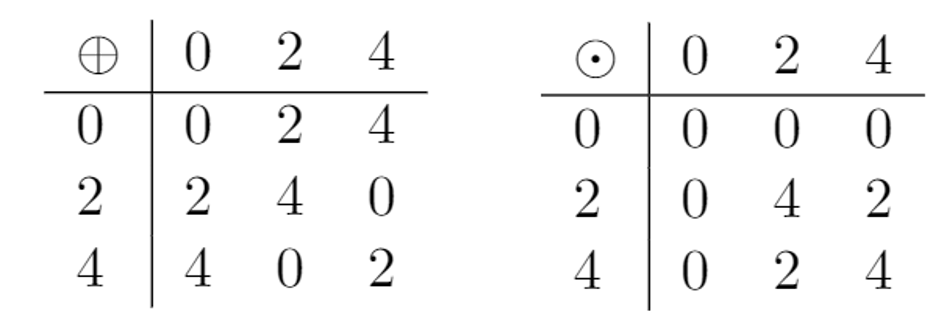
\includegraphics[width=2.3in]
	         {images/newCayleyTables.png}}
\end{figure}

Since all the rows and columns have all the elements $\{0,2,4\}$ in the modular addition and modular multiplication tables, then all four subring properties are satisfied and  $\{0,2,4\}$ is a subring of ${\mathbb Z}_6$\\
\end{proof}
\end{example}

We can generalize this idea with the following exercise.

\begin{exercise}{}
If $R={\mathbb Z}_{mn}$ and $S=\{0,m,2m,...(n-1)m\}$, then $S$ is a subring of $R$ without unity. (${\mathbb Z}_6={\mathbb Z}_{mn}$, where $m=2$ and $n=3$.)  
\end{exercise}

\section{Extension Rings}
\label{sec:extensionRings}

We have learned that a subring can be formed from a subset of a ring. One example we used was that $\{0,2,4\}$ is a subring of ${\mathbb Z}_6$. We can also extend a ring into a larger set, called an extension ring.  We would say that ${\mathbb Z}_6$ is an extension ring of $\{0,2,4\}$.

\begin{defn}\label{ext_ring}
If $R$ is a subring of $S$, then we can say that $S$ is an \term{extension ring} of $R$.
\end{defn}

Extension rings  can be used to create number systems that are more "complete" in some sense. In fact, you've seen extension rings several times before. The integers form a very simple number system, but integers lack multiplicative inverses. The set of rational numbers is in fact an extension ring of the integers, which includes the multiplicative inverses that integers lack.  Similarly, real numbers are "incomplete" in the sense that some real numbers do not have roots (e.g. there is no real square root of -1).  The complex numbers form a larger number system that includes the real numbers, and also has the missing roots. 

Another example of extension ring that we've seen before is the polynomial ring ${\mathbb Q}[x]$, which contains the ring ${\mathbb Q}$. Some polynomials lack multiplicative inverses as the following proposition shows.

\begin{prop}{}
$p(x)=1+x$ has no multiplicative inverse in ${\mathbb Q}[x]$.

\begin{proof}
We will show by contradiction that $1 + x$ has no  multiplicative inverse in 
${\mathbb Q}[x]$. Suppose on the contrary that $1+x$ has an inverse that can be written as $q(x) = \sum_{n=0}^{N}a_nx^n$, where $a_N$ is the leading nonzero coefficient and $N \ge 0$. Then 
\begin{equation*}
(1+x)q(x) = (1+x) \cdot \sum_{n=0}^{N}a_nx^n=a_{N}x^{N+1}+\cdots+a_0.
\end{equation*}
Since $a_N \neq 0$, it follows that the degree of $(1+x)q(x)$ is equal to $N+1$, so it is not a constant polynomial.  In particular, $(1+x)q(x) \neq 1$. This contradicts the supposition that $q(x)$ is the multiplicative inverse of $1+x$. Therefore, $(1+x)$ does not have a  multiplicative inverse in ${\mathbb Q}[x]$. 
\end{proof}
\end{prop}

We can actually go further, and take infinite power series in addition to finite polynomials. This gives us an even larger extension ring:

\begin{example}{powerSeriesRing}
Let $\widehat{{\mathbb Q}}[x]$ be the set of power series with rational coefficients:
\begin{align*}
\widehat{{\mathbb Q}}[x]=\{\sum_{n=0}^{\infty}a_n x^n\}~\text{, where}~a_n\in {\mathbb Q}.\\  
\text{Show that}~ \widehat{{\mathbb Q}}[x]~\text{is an extension ring of}~{\mathbb Q}[x].
\end{align*}
Now, the question is does $p(x)$ have a multiplicative inverse in $\widehat{{\mathbb Q}}[x]$? There are 3 methods we can do to figure this out.
\begin{enumerate}
\item Taylor series
\item Long division
\item Linear recurrence relation
\end{enumerate}

We will explore all three methods in the following example.

\begin{example}{Zx}
Find the multiplicative inverse of $(1+x)$ in $\widehat{{\mathbb Z}}[x]$\\

\begin{enumerate}
\item First Method: Taylor series

The Taylor series expansion for the function $f(x)$ about the point $a=0$ is given by:
\begin{equation*}{}
f(x)=f(0)+f'(0)x+\frac{f''(0)x^2}{2!}+\frac{f'''(0)x^3}{3!}+\cdots
\end{equation*}
For $f(x)=\frac{1}{1+x}$ , we have:
\begin{align*}
\left(\frac{1}{1+x}\right)'&=((1+x)^{-1})'=-1!(1+x)^{-2}\implies \text{when $x=0,~f'(x)=-1$}\\
((1+x)^{-1})''&=-1(-2)(1+x)^{-3}=2!(1+x)^{-3}\implies \text{when $x=0,~f''(x)=2$}\\
((1+x)^{-1})'''&=2(-3)(1+x)^{-4}=-3!(1+x)^{-4} \implies \text{when $x=0,~f'''(x)=-3$}\\
\text{In general:} \\
((1+x)^{-1})^{(n)}&=(-1)^{n}n!(1+x)^{-n-1} \implies \text{when $x=0,~f^n(x)=(-1)^{n}n!$}
\end{align*}
Therefore,
\begin{equation}
(1+x)^{-1}=1-x+x^2-x^3+\cdots=\sum_{n=0}^{\infty}(-1)^nx^n\in \widehat{{\mathbb Q}}[x]
\end{equation}
This is a multiplicative inverse of $(1+x)$ in $\widehat{{\mathbb Z}}[x]$ (also in $\widehat{{\mathbb Q}}[x]$).

\item Second Method: Long Division\\

Use long division to divide $\frac{1}{1+x}:$\\ 

\begin{tabular}{cccccccccccc}
&  $1$ & $-$ & $x$ & $+$ & $x^2$ & $-$ & $x^3$ & $+$ & $\cdots$\\ \cline{2-10}

\multicolumn{1}{r|}{$1 + x$}
&  $1$ & $+$ & $0x$ & $+$ & $0x^2$ & $+$ & $0x^3$ & $+$ & $\cdots$\\
& $-1$ & $+$ & $-x$\\ \cline{2-4}
&      &     & $-x$ & $+$ & $0x^2$\\ 
&      &     & $+x$ & $+$ & $x^2$\\ \cline{4-8}
&      &     &      &     & $x^2$ & $+$ & $0x^3$\\ 
&      &     &      &     & $-x^2$ & $-$ & $x^3$\\ \cline{6-8}
&      &     &      &     &       &        & $-x^3$ & $+$ &  $\cdots$\\
&      &     &      &     &       &        &        & $\vdots$\\

\end{tabular}

\item Third Method: Linear Recurrence Relation:\\

We want:

\begin{equation*}{}
1=(a+x)\sum_{n=0}^{\infty}a_nx^n=1+0x+0x^2+\cdots
\end{equation*}
%%%% Should I call this the distributive property?
Use distributive law:

\begin{align*}
1&=a\sum_{n=0}^{\infty}a_nx^n+x\sum_{n=0}^{\infty}a_nx^{n}  & \text{distributive law}\\
&=\sum_{n=0}^{\infty}a_nx^n+\sum_{n=0}^{\infty}a_nx^{n+1} & \text{simplify}\\
&=\sum_{n=0}^{\infty}a_nx^n+\sum_{n=1}^{\infty}a_{n-1}x^{n} & \text{change second summation index}\\ 
&=a_0+\sum_{n=1}^{\infty}a_nx^n+\sum_{n=1}^{\infty}a_{n-1}x^{n} & \text{separate one term from sum}\\
&=a_0+\sum_{n=1}^{\infty}(a_nx^n+a_{n-1}x^n) & \text{combine two sums}\\
&=a_0+\sum_{n=1}^{\infty}(a_n+a_{n-1})x^n & \text{factor out $x_n$}\\
\end{align*}
Now we can write:
\begin{align*}
1+0x+0x^2+\cdots=a_0+\sum_{n=1}^{\infty}(a_n+a_{n-1})x^n\\
\end{align*}

Equate like powers of $x$ for the two polynomials:
\begin{align*}
1&=a_0\\
0&=a_1+a_0=a_1+1\implies a_1=-1\\
0&=a_2+a_1=a_2+-1\implies a_2=1\\
0&=a_3+a_2=a_3+1\implies a_3=-1\\
0&=a_4+a_3=a_4+-1\implies a_4=1\\
\vdots\\
0&=a_n+a_{n-1}\implies a_n=(-1)^n
\end{align*}
\end{enumerate}
\end{example}

\begin{exercise}{}
Find the inverse of $a+x$ in $\widehat{{\mathbb Q}}[x]$ by the:
\begin{enumerate}
\item long division method
\item recurrence relation method
\end{enumerate}
\end{exercise}

\begin{exercise}{Z2x}
Find the inverse of $1+x$ in $ \widehat{{\mathbb Z}}_{2}[x]$ by the:
\begin{enumerate}[(a)]
\item long division method
\item recurrence relation method
\end{enumerate}
\end{exercise}

\begin{exercise}{}
Find the inverse of $3+2x$ in $ \widehat{{\mathbb Z}}_{5}[x]$ by the:
\begin{enumerate}[(a)]
\item long division method
\item recurrence relation method
\end{enumerate}
\end{exercise}

\begin{exercise}{Z5x}
Find the multiplicative inverse of $(1+2x+3x^2)$ in $ \widehat{{\mathbb Z}}_5[x]$, in $ \widehat{{\mathbb Z}}_7[x]$, and in $ \widehat{{\mathbb Q}}[x]$ by the:
\begin{enumerate}[(a)]
\item long division method
\item recurrence relation method
\end{enumerate}
\end{exercise}
\end{example}

\section{Product Rings}
\label{sec:ProductRings}

In certain situations, we may want to combine two or more rings to form a larger ring. Product rings allow us to do just that. In fact, the product operation for rings is very similar to the product of groups (see Definition~\ref{def:ProductOfGroups}).

\begin{defn}\label{product ring}
If $R_1,~R_2$ are rings, then the \emph{product ring}, $R_1\times R_2$ is the set of pairs $(a,b),~a\in R_1$ and $b\in R_2$, with the following operations:
\begin{enumerate}
\item $(a,b)+(c,d)=(a+_1c,b+_2d)$
\item $(a,b)\cdot(c,d)=(a\cdot_1c,b\cdot_2d)$
\end{enumerate}
where $+_1,\cdot_1$ is the addition and multiplication for $R_1$ and $+_2,\cdot_2$ is the addition and multiplication for $R_2$\\
\end{defn}
How do we know that the product ring is a ring? As with any ring, we must show that the seven ring properties hold true.

\begin{proof}
\begin{enumerate}[(I)]
\item Closure: 
\begin{enumerate}[(a)]
\item Additive closure: If $(a,b)$, and $(c,d)$ are in $R_1\times R_2$, then $(a,b)+(c,d)$ is also in $R_1\times R_2$.
\begin{align*}
(a,b)+(c,d)&=(a+_1c,b+_2d) & \text{Def. of product add.}\\
a+_1 c \in R_1 & \text{ and } b+_2d\in R_2 & \text{Closure of } R_1, R_2\\
(a+_1c,b&+_2d)\in R_1\times R_2 & \text{Definition of }R_1\times R_2
\end{align*}
\item Multiplicative closure: If $(a,b)$ and $(c,d)$ are in $R_1\times R_2$, then $(a,b)(c,d)$ is also in $R_1\times R_2$.
\begin{align*}
(a,b)(c,d)&=(a\cdot_1 c, b\cdot_2 d) & \text{Def. of product mult.}\\
a\cdot_1c\in R_1 & \text{ and }b\cdot_2d\in R_2 & \text{Closure of $R_1$ and $R_2$}\\
(a\cdot_1c,b&\cdot_2d)\in R_1\times R_2 & \text{Definition of $R_1\times R_2$} 
\end{align*}
\end{enumerate}
\item Associativity:
\begin{enumerate}[(a)]
\item Associativity of Addition:  For $(a,b),(c,d),(e,f)\in R_1\times R_2$,\\ 
$((a,b)+(c,d))+(e,f)=(a,b)+((c,d)+(e,f)$.\\

$((a,b)+(c,d))+(e,f)$
\begin{align*}
&=((a+_1c)+_1e,(b+_2d)+_2f) & \text{Def. of product add.}\\
&=(a+_1(c+_1e),b+_2(d+_2f)) & \text{Assoc. of add. in $R_1\times R_2$}\\
&=(a,b)+((c,d)+(e,f)) & \text{Def. of product additon}
\end{align*}
\item Associativity of Multiplication:  For $(a,b),(c,d),(e,f)\in R_1\times R_2$,\\   
$((a,b)(c,d))(e,f) = (a,b)((c,d)(e,f))$.

We leave this part of the proof as an exercise.
\end{enumerate}

\begin{exercise}{}
Prove the associative property of multiplication for $R_1 \times R_2$.
\end{exercise}
\item Commutativity of Addition:  For all $a,b,c\in R_1\times R_2$,\\ 
$(a,b)+(c,d)=(c,d)+(a,b).$
\begin{align*}
(a,b)+(c,d)&=(a+_1c,b+_2d) & \text{Definition of product addition}\\
&=(c+_1a,d+_2b) & \text{Commutativity of $+_1$ and $+_2$}\\
&=(c,d)+(a,b) & \text{Definition of product addition}
\end{align*}
\item Zero: Show that the additive identity for $R_1\times R_2$ is $(0_1,0_2)$.
\begin{align*}
(a,b)+(0_1,0_2)&=(a+_10_1,b+_20_2) & \text{Definition of product addition}\\
&=(a,b) & \text{Additive identities for $R_1$ and $R_2$}\\
(0_1,0_2)+(a,b)&=(a,b) & \text{(similar to above)}
\end{align*}
\item One: Show that the multiplicative identity for $R_1\times R_2=(1_1,1_2)$.

The proof of this property is left as an exercise.

\begin{exercise}{}
Prove that the multiplicative identity for $R_1\times R_2=(1_1,1_2)$.
\end{exercise}

\item Additive inverse:  The additive inverse of $(a,b)=(-a,-b)$.
\begin{align*}
(a,b)+(-a,-b)&=(a+_1-a,b+_2-b) & \text{Def.  of product addition}\\
&=(0_1,0_2) & \text{Additive inverses of $R_1$ and $R_2$}\\
&=\text{additive~identity~of}~R_1\times R_2 & \text{proven in part(IV)}
\end{align*}
\item Distributive property:  For $(a,b),(c,d),(e,f) \in  R_1 \times R_2$:
\begin{itemize}
\item $(a,b)((c,d)+(e,f)) = (a,b)(c,d)+(a,b)(e,f)$ and 
\item $((c,d)+(e,f))(a,b) = (c,d)(a,b)+(e,f)(a,b)$.
\end{itemize}
\begin{exercise}{}
Prove the distributive property for the product ring $R_1 \times R_2$.
\end{exercise}
\end{enumerate}
\end{proof}

\begin{exercise}{}
Give the addition and multiplication tables for the following product rings:
\begin{enumerate}
\item ${\mathbb Z}_2\times {\mathbb Z}_2$ with elements: $\{(0,0),(0,1),(1,0),(1,1)\}$ 
\item $({\mathbb Z}_2\times {\mathbb Z}_2)\times {\mathbb Z}_2$ with elements: $\{0,0,0),(0,0,1),etc\}$
\item ${\mathbb Z}_2\times {\mathbb Z}_3$ (6 elements)
\end{enumerate}
\end{exercise}

\section{Isomorphic rings}
\label{sec:IsomorphicRings}

Sometimes we encounter rings that are basically the ``same''.  In this section we will give a mathematical definition for what the ``same'' means in this context.  Before we give the definition, we will start out with an example.

\begin{example}{}
Consider the two rings $R_1={\mathbb Z}[x]$ and $R_2={\mathbb Z}[y]$.  Obviously, these two rings are basically the same except we replace $x$ with $y$.  We can make a formal correspondence between the two rings by defining a function $\phi:R_1\rightarrow R_2$ as follows: $\phi(a_nx^n+a_{n-1}x^{n-1}+\ldots +a_0)=(a_ny^n+a_{n-1}y^{n-1}+\ldots +a_0)$.  Note that $\phi$ is a bijection because it has an inverse (see Proposition \ref{proposition:functions:InverseBijection}).  Additionally, $\phi$ preserves the operations of addition and multiplication:  $\phi(x+_1y)=\phi(x)+_2\phi(y)$ and
$\phi(x\cdot_1y)=\phi(x)\cdot_2\phi(y)$.  In other words, $\phi$ gives us a way to ``translate'' every operation we do in $R_1$ to a corresponding operation in $R_2$.
\end{example}
The above example may seem trivial, but it turns out that in some cases similar construction can make deep connections between rings that seem quite different:

\begin{example}{phi_matrix}
Consider the function $\phi:R_1\rightarrow R_2$, where\\
$R_1=\{z=a+bi\in{\mathbb C}\}$, $R_2=\left\{A=
\begin{bmatrix}
a & b\\
-b & a
\end{bmatrix}\in{\mathbb M}_2\right\}$ and $\phi$ is defined as:
$\phi(a+bi)=
\begin{bmatrix}
a & b\\
-b & a
\end{bmatrix}$.
We can see that $\phi$ is also a bijection since $\phi^{-1}\left(
\begin{bmatrix}
a & b\\
-b & a
\end{bmatrix}\right)
=a+bi$, for all
$A\in R_2$.\\

To further explore the structure of the function $\phi$, let's consider two arbitrary elements of $R_1$, say $z=a+bi$ and $w=c+di$.  Using addition of complex numbers, then applying the $\phi$ function, we get
\begin{align*}
\phi(z+w)&=\phi(a+bi+c+di)\\
&=\phi((a+c)+(b+d)i)\\
&=
\begin{bmatrix}
a+c & b+d\\
-b-d & a+c
\end{bmatrix}.
\end{align*}
We get the same result if we first apply the $\phi$ function on $z$ and $w$, then use addition of matrices:
\begin{align*}
\phi(z)+\phi(w)&=\phi(a+bi)+\phi(c+di)\\
&=
\begin{bmatrix}
a & b\\
-b & a
\end{bmatrix}+
\begin{bmatrix}
c & d\\
-d & c
\end{bmatrix}\\
&=
\begin{bmatrix}
a+c & b+d\\
-b-d & a+c
\end{bmatrix}.
\end{align*}
In other words, $\phi(z+_1w)=\phi(z)+_2\phi(w)$, where $+_1$ and $+_2$ are addition as defined by $R_1$ and $R_2$, respectively.  But what about multiplication?

Let's consider $z$ and $w$ as defined earlier.  We can see that
\begin{align*}
\phi(z\cdot w)&=\phi((a+bi)\cdot(c+di))\\
&=\phi((ac-bd)+(ad+bc)i)\\
&=
\begin{bmatrix}
ac-bd & ad+bc\\
-ad-bc & ac-bd
\end{bmatrix}.
\end{align*}
Note that multiplication of complex numbers was used here.  Also,
\begin{align*}
\phi(z)\cdot\phi(w)&=\phi(a+bi)\cdot\phi(c+di)\\
&=
\begin{bmatrix}
a & b\\
-b & a
\end{bmatrix}\cdot
\begin{bmatrix}
c & d\\
-d & c
\end{bmatrix}\\
&=
\begin{bmatrix}
ac-bd & ad+bc\\
-ad-bc & ac-bd
\end{bmatrix}, 
\end{align*}
where multiplication of matrices was used.  So, $\phi(z\cdot_1 w)=\phi(z)\cdot_2\phi(w)$, where $\cdot_1$ and $\cdot_2$ are multiplication as defined by $R_1$ and $R_2$, respectively.   
\end{example}
The two examples above show how we can relate different rings that have the same structure. In both examples we use a bijection that preserves the addition and multiplication operations to make a correspondence between two rings. We may generalize this type of bijection as follows.

\begin{defn}\label{Isomorphism}
Let $\phi:R_1\rightarrow R_2$ be a bijection between rings $R_1$ and $R_2$.  We say that $\phi$ is an \term{isomorphism} from $R_1$ to $R_2$ if the following two equations are satisfied for all $x,y\in R_1$:
\begin{equation}\label{iso_add}
\phi(x+_1y)=\phi(x)+_2\phi(y)
\end{equation}
\begin{equation}\label{iso_mult}
\phi(x\cdot_1y)=\phi(x)\cdot_2\phi(y)
\end{equation}.

Two rings $R_1$ and $R_2$ are called \term{isomorphic} if there exists an isomorphism from $R_1$ to $R_2$.
\end{defn}

\begin{exercise}{}
Show that isomorphism is an equivalence relation on rings: that is show that isomorphism satisfies the reflexive, symmetric and transitive properties.
\end{exercise}

\begin{exercise}{matrixIso}
Let $\phi: R_1\rightarrow R_2$, where $R_1={\mathbb Q}[\sqrt{2}]=\{a+b\sqrt{2}:  a,b\in{\mathbb Q}\}$ and $R_2=\left\{
\begin{bmatrix}
a & b \sqrt{2}\\
b \sqrt{2} & a
\end{bmatrix}
\in{\mathbb M}_2\right\}$.  Prove or disprove that $\phi$ is an isomorphism.
\end{exercise}

\begin{example}{conjugate}
Show that $f:{\mathbb C}\rightarrow{\mathbb C}$ is an isomorphism, where $f$ maps every element of ${\mathbb C}$ to its complex conjugate in ${\mathbb C}$.  In other words, if $z=a+bi\in{\mathbb C}$, where $a,b\in{\mathbb R}$, then $f(z)=a-bi\in{\mathbb C}$.

\begin{proof}{}
In order for $f$ to be an isomorphism, we must first show that the sets are indeed rings and that the function $f$ is a bijection.  Then we must show that the two equations above are true for all $z,w\in{\mathbb C}$.  At the beginning of this chapter, we concluded that ${\mathbb C}$ satisfies all seven properties of a ring.  Also, given any $w=a-bi\in{\mathbb C}$, $f^-1(w)=a+bi\in{\mathbb C}$.  So $f$ is a bijection.\\  
As we continue, remember that $+_1, \cdot_1$ and $+_2, \cdot_2$ refer to addition and multiplication as defined by the first and second rings, respectively.  In our case, both additions are regular complex addition and both multiplications are regular complex multiplication.  So we will use $+$ to represent both $+_1$ and $+_2$ and similarly for $\cdot$.
\begin{enumerate}[(1)]
\item First we must show that $f(z+w)=f(z)+f(w)$, for any $z,w\in{\mathbb C}$.  We begin with our two arbitrary elements of ${\mathbb C}$, $z=a+bi$ and $w=c+di$, where $a,b,c,d\in{\mathbb R}$.  Then 
\begin{align*}
f(z+w)&=f((a+bi)+(c+di)\\
&=f((a+c)+(b+d)i)\\
&=(a+c)-(b+d)i\\
&=a+c-bi-di\\
&=(a-bi)+(c-di)\\
&=f(z)+f(w).
\end{align*}
So property one of isomorphisms is satisfied.
\item Secondly, we must show that $f(z\cdot w)=f(z)\cdot f(w)$.  Using $z$ and $w$ as defined above,

\begin{align*}
  f(z\cdot w)&=f((a+bi)\cdot(c+di))\\
  &=f((ac-bd)+(ad+bc)i)\\
  &=(ac-bd)-(ad+bc)i.
\end{align*}
On the other hand,
\begin{align*}
f(z)\cdot f(w)&=f(a+bi)\cdot f(c+di)\\
&=(a-bi)(c-di)\\
&=(ac-bd)-(ad+bc)i
\end{align*}
This shows $f(z\cdot w)=f(z)\cdot f(w)$, so property two of isomorphisms is satisfied.
\end{enumerate}
\end{proof}
\end{example}

Note that there can be more than one isomorphism between two rings.

\begin{exercise}{}
In Example \ref{example:rings:conjugate} we gave an isomorphism from ${\mathbb C}$ to itself.  Give another example of an isomorphism from ${\mathbb C}$ to itself.  (\emph{Hint}:  Make your example as easy as possible.)
\end{exercise}

\begin{exercise}{phi_iso}
Given $\phi:  {\mathbb Q}[x,y]\rightarrow{\mathbb Q}[x,y]$, defined by $\phi(p(x,y))=p(y,x)$:
\begin{enumerate}[(a)]
\item Show that $\phi$ is an isomorphism.
\item Give another isomorphism between ${\mathbb Q}[x,y]$ and ${\mathbb Q}[x,y]$.
\end{enumerate}
\end{exercise}

When we restrict the isomorphism, so that $R_1=R_2$, we have a special type of isomorphism known as an \emph{automorphism}.

\begin{defn}\label{automorphism}
A \term{ring automorphism} is a ring isomorphism whose domain is equal to its range.
\end{defn}

\begin{example}{}
Show that $f(a+bi)=a-bi$ is a ring automorphism from ${\mathbb C}$ to ${\mathbb C}$.

We showed in Example \ref{example:rings:conjugate} that this function is a ring isomorphism.  It should be clear that the domain and range of $f$ are the same, so $f$ is also a ring automorphism.  
\end{example}

\begin{exercise}{abc_iso}
Consider the function $f((a,b,c))=(a,-b,c)$, where $a,b,c\in{\mathbb R}$.
\begin{enumerate}[(a)]
\item show that f is a homomorphism by proving that:
\begin{enumerate}[(1)]
\item $f((a,b,c)+(d,e,f))=f((a,b,c))+f((d,e,f))$, and 
\item $f((a,b,c)\cdot(d,e,f))=f((a,b,c))\cdot f((d,e,f))$.
\end{enumerate}
\item Is $f$ an isomorphism? \hyperref[ringsHints]{(*Hint*)} 
\item Is $f$ an automorphism?
\end{enumerate}
\end{exercise}

\section{Ring homomorphisms: kernels, and ideals}
\label{sec:RingHomomorphismKernelsIdeals}

As we have seen above, ring isomorphisms are functions that are bijections and preserve the additive and multiplicative operations. It is possible to have functions that are not bijections but still preserve the additive and multiplicative operations.  One important example is a function that we are very familiar with: 

\begin{example}{ring_homo}
Define the function $f:{\mathbb Z}\rightarrow {\mathbb Z}_n$ defined by $f(x)=\bmod(x,n)$, where $n$ is a fixed integer $> 1$.  In Proposition~\ref{proposition:modular:number_remainder} we showed that for any $\ell,m \in {\mathbb Z}$ we have:
\begin{enumerate}[(a)]
\item
$\bmod(\ell+ m,n) = \bmod(\ell,n) \oplus \bmod(m,n)$, 
and
\item
$\bmod(\ell \cdot m,n) = \bmod(\ell,n) \odot \bmod(m,n)$.
\end{enumerate}
We may rewrite these equations in terms of $f$ as $f(\ell+ m) = f(\ell) \oplus f(m)$ and $f(\ell\cdot m) = f(\ell) \odot f(m)$. 
\end{example}
We may generalize this example with the following definition.

\begin{defn}\label{homomorph}
A function $f:R_1\rightarrow R_2$ between rings $R_1,R_2$ is called a \term{ring homomorphism} if $f$ has the following properties:
\begin{equation}\label{eq:homo_add}
f(\ell+_1 m) = f(\ell) +_2 f(m)
\end{equation} 
\center{and} 
\begin{equation}\label{eq:homo_mult}
f(\ell\cdot_1 m) = f(\ell) \cdot_2 f(m).
\end{equation}
\end{defn}
Notice that a homomorphism is an isomorphism without the bijection requirement.  Figure \ref{fig:ring_functions} shows the relationship between homomorphisms, isomorphisms and automorphisms.

\begin{figure}[H]
\begin{center}
\centerline {
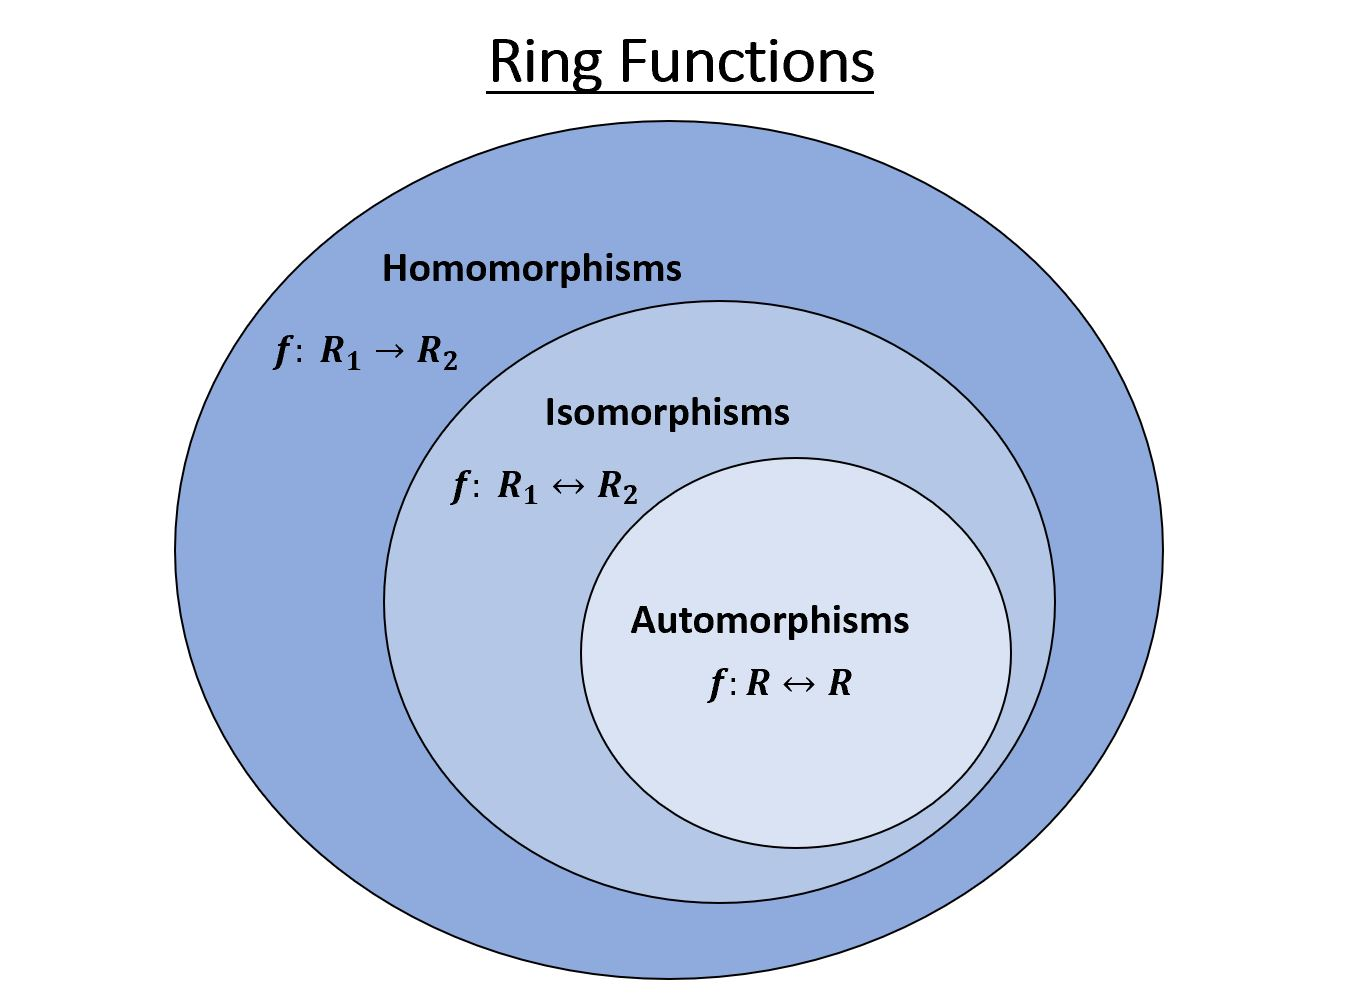
\includegraphics[width=4in]{images/ringFunctions.jpg} }
\end{center}
\caption{Ring Functions}\label{fig:ring_functions}
\end{figure}

Following are a number of examples of ring homomorphisms.

\begin{example}{notHomo}
Prove or disprove that $f:{\mathbb Q}\rightarrow {\mathbb Q}$ defined by : $f(x)=2x$ is a ring homomorphism.

\begin{proof}
$f$ is \emph{not} a homomorphism since it does not follow Equation \ref{eq:homo_mult}:\\
For example, $f(1\cdot1)=2(1\cdot 1)=2$ but $f(1)+f(1)=2(1)\cdot 2(1)=4$.  Many other counterexamples can be found.\\
\end{proof}
\end{example}

\begin{example}{homo}
Prove or disprove that  $f:{\mathbb Z}_6\rightarrow {\mathbb Z}_3$ defined by: $f(x)=\bmod(x,3)$ is a ring homomorphsm.\\

\begin{proof}
$f$ is a homomorphism since,
\begin{align*}
f(x+_6y)&=\bmod(x+_6y,3)=\bmod(x,3)+_3\bmod(y,3),\\
&\text{ where } +_n \text{ is addition in } {\mathbb Z}_n, \text{ and}\\
f(x\cdot_6y)&=\bmod(x\cdot_6y,3)=\bmod(x,3)\cdot_3\bmod(y,3),\\ &\text{ where } \cdot_n \text{is multiplication in } {\mathbb Z}_n
\end{align*}
\end{proof}
\end{example}

\begin{exercise}{homo}
Given integers $m,n>1$, define $g:{\mathbb Z}_{mn}\rightarrow {\mathbb Z}_n$ defined by $g(x)=\bmod(x,n)$.  Show that $g$ is a homomorphism.
\end{exercise}

\begin{example}{polyhom}
Prove or disprove that $f:{\mathbb R}[x]\rightarrow{\mathbb R}$, defined by $f(p(x))=p(0)$, is a homomorphism.  (Note that this function maps a polynomial to its constant term.)

\begin{proof}
We will divide this proof into two parts, one for each property of ring homomorphisms:
\begin{enumerate}[(a)]
\item Let $p(x),q(x)$ be arbitrary elements of ${\mathbb R}[x]$, where $p(x)$ and $q(x)$ have constant terms of $a_0,b_0\in {\mathbb R}$, respectively.  Then $p(x)+_1q(x)$ is some polynomial in ${\mathbb R}[x]$, with a constant term equal to $a_0+b_0$.  So,
\begin{align*}
f(p(x)+_1q(x))&=a_0+b_0.\\
\text{Also, } f(p(x))+_2f(q(x)&)=a_0+b_0.
\end{align*}
The first ring homomorphism property holds.  Let's look at the second property:
\item  $p(x)\cdot_1q(x)$ is some polynomial in ${\mathbb R}[x]$, with a constant term equal to $a_0\cdot b_0$.  So,
\begin{align*}
f(p(x)\cdot_1q(x))&=a_0\cdot b_0.\\
\text{Also, }f(p(x))\cdot_2f(q(x))&=a_0\cdot b_0.
\end{align*}
So, the second ring homomorphism property holds and we can say that $f$ is a ring homomorphism.
\end{enumerate}
\end{proof}
\end{example}
The homomorphism in Example \ref{example:rings:polyhom} is just one example of an important class of homomorphisms.  

\begin{exercise}{}
Give $a\in{\mathbb Q}$ define the function $f_a:  {\mathbb Q}[x]\rightarrow{\mathbb Q}$ by\\ $f_a(p(x))=p(a)$.  For what values of $a$ is $f_a$ a homomorphism?
\end{exercise}

\begin{exercise}{R_C_homo}
Define the function $f:{\mathbb R}[x]\rightarrow C_3({\mathbb R})$ by
\[f(a_nx^n+a_{n-1}x^{n-1}+\cdots +a_0)=a_nB^n+a_{n-1}B^{n-1}+\cdots +a_0,\] 
where $B=
\begin{bmatrix}
0 & 0 & 1\\
1 & 0 & 0\\
0 & 1 & 0
\end{bmatrix}.$

\begin{enumerate}[(a)]
\item Show that $f$ is onto.  You may show this by showing that for any matrix $A\in C_3({\mathbb R})$ there exists some $p(x)\in {\mathbb R}[x]$ such that $f(p(x))=A$.
\end{enumerate}
\end{exercise}



\subsection{Homomorphism kernels and ideals}

When we discussed homomorphisms of groups, we introduced the notion of the kernel of a homomorphism.  According to Definition \ref{def:kernel}, the kernel of a group homomorphism is the inverse image of the identity element of the codomain.  We may make a similar definition for ring homomorphisms.  

\begin{defn}\label{kernel}
If $f:R_1\rightarrow R_2$ is a ring homomorphism, then the set $\{x\in R_1|f(x)=0\}$ is called the \term{kernel} of $f$, notated $Ker(f)$.
\end{defn}

\begin{example}{}
Find the kernel of $f:{\mathbb R}[x]\rightarrow{\mathbb R}$, given by$f(p(x))=p(0)$.

We are looking for the set of all $p(x)$ such that $p(0)=0$. 
We know from the polynomials chapter that $p(0)=0$ implies that $x$ divides $p(x)$.  (So, there is no constant term!)  In summary, $Ker(f)=\{xp(x): p(x)\in{\mathbb R}[x]\}$.
\end{example}

\begin{exercise}{}
Given $f_a:{\mathbb Q}[x]\rightarrow{\mathbb Q}$, where $f_a(p(x))=p(a)$.  Find $Ker(f_a)$.
\end{exercise}

\begin{exercise}{}
In Exercise \ref{exercise:rings:R_C_homo}, we defined a function $f:{\mathbb R}[x]\rightarrow C_3({\mathbb R})$.
\begin{enumerate}[(a)]
\item For what values of $a$ is $x^3+a$ in $Ker(f)$?
\item Consider the polynomial $p(x)=(x^3-1)\cdot q(x)+a_2x^2+a_1x+a_0$.  Show that $p(x)\in Ker(f)$ if and only if $a_0=a_1=_2=0$.
\end{enumerate}
\end{exercise}

We saw previously that the kernel of a group homomorphism is always a subgroup of the domain (see Proposition \ref{proposition:homomorph:homo_ker_normal}).  We may ask the same question of rings:  Given a ring homomorphism $f$, is $Ker(f)$ also a ring?

\begin{exercise}{}
\begin{enumerate}[(a)]
    \item Given the homomorphism $f$ defined in Example~\ref{example:rings:ring_homo}, show that $f^{-1}(0)$ is \emph{not} a ring.  Which properties fail?
    \item Given the same example, show that $f^{-1}(1)$ is \emph{also not} a ring.  Which ring properties fail?
\end{enumerate}
\end{exercise}

Although the set $f^{-1}(0)$ is not a ring, nonetheless it does have some nice properties.

\begin{exercise}{kernel_props}
Given the function $f$ defined in Example~\ref{example:rings:ring_homo}, and let $S=f^{-1}(0)$.
\begin{enumerate}[(a)]
\item Show that if $a,b \in S$, then $a+b \in S$.  In other words, $S$ is closed under addition.
\item Show that if $a,b \in S$, then $a\cdot b \in S$.  In other words, $S$ is closed under multiplication.

\item Show that if $a \in S$, then $-a \in S$.  In other words, $S$ is closed under additive inverse.
\end{enumerate}
\end{exercise}

The following proposition generalizes the results in Exercise \ref{exercise:rings:kernel_props}.

\begin{prop}{kernelIsIdeal}
The kernel of a homomorphism $f:R_1\rightarrow R_2$ satisfies the following properties:
\begin{enumerate}
\item If $a,b\in f^{-1}(0)$, then $a+b\in f^{-1}(0)$.
\item If $a\in f^{-1}(0)$ and $b\in R_1$ then $ab\in f^{-1}(0)$.
\item $0\in f^{-1}(0)$.
\item If $a\in f^{-1}(0)$, then $-a\in f^{-1}(0)$.
\end{enumerate}

\begin{proof}
\begin{enumerate}
\item
\begin{align*}
&a,b\in f^{-1}(0) & \text{given}\\
&f(a)=0,f(b)=0 & \text{def. of inverse}\\
&f(a+b)=f(a)+f(b) & \text{def. of homomorphism}\\
&f(a+b)=0+0=0 & \text{substitution \& zero property}\\
&a+b\in f^{-1}(0) & \text{def. of inverse}
\end{align*}
\item
\begin{align*}
&a\in f^{-1}(0),~b\in R_1 & \text{given}\\
&f(a)=0 & \text{def. of inverse}\\
&f(a\cdot b)=f(a)\dot f(b) & \text{def. of homomorphism}\\
&f(a\cdot b)=0\cdot f(b)=0 & \text{substitution \& Prop. \ref{proposition:rings:add_inverse}}\\
&ab\in f^{-1}(0) & \text{def. of inverse}
\end{align*}
\item
\begin{align*}
f(a)&=f(a+0) & \text{additive identity}\\
f(a+0)&=f(a)+f(0) & \text{def. of homomorphism}\\
f(a)&=f(a)+f(0) & \text{substitution}\\
-f(a)+f(a)&=-f(a)+f(a)+f(0) & \text{substitution}\\
0&=0+f(0) & \text{additive inverse}\\
0&=f(0) & \text{additive identity}\\
0&\in f^{-1}(0) & \text{def. of inverse}
\end{align*}
\item
\begin{align*}
&a\in f^{-1}(0) & \text{given}\\
&f(a)=0 & \text{def. of inverse}\\
&-a\in R_1 & \text{def. of homomorphism}\\
f(0)&=f(a+(-a)) & \text{additive inverse}\\
f(0)&=f(a)+f(-a) & \text{def. of homomorphism}\\
f(0)&=0 & \text{proven above}\\
0&=0+f(-a) & \text{substitution}\\
0&=f(-a) & \text{additive identity}\\
-a&\in f^{-1}(0) & \text{def. of inverse}
\end{align*}
\end{enumerate}
\end{proof}
\end{prop}

Any set $J$ which has properties (1-4) is called an \textit{ideal}.  We formalize the definition of ideal as follows.

\begin{defn}\label{def:ideal}
Given a ring $R$, suppose $J \subset R$ satisfies the following properties:
\begin{enumerate}[(a)]
\item $J$ is closed under the ring's additive operation:  in other words if $j_1,j_2\in J$ then $j_1+j_2\in J$.
\item $J$ is closed under multiplication by elements in $R$:  in other words, if $j\in J$ and $r\in R$ then $rj\in J$.
\item $J$ is closed under additive inverse in $R$.
\end{enumerate}
Then $J$ is called an \term{ideal} of $R$.
\end{defn}

\begin{exercise}{}
In Example we showed the property that for any homomorphism $f:R_1\rightarrow R_2$, we have $0_1\in Ker(f)$.  Using Definition \ref{def:ideal}, show that for any ideal $J$ the zero element is an element of $J$. 
\end{exercise}

In view of Definition \ref{def:ideal}, we may restate Proposition \ref{proposition:rings:kernelIsIdeal} as follows.

\begin{prop}{kernel_ideal}
The kernel of a homomorphism is always an ideal.
\end{prop}

\begin{exercise}{}
Find the kernel for the functions in Examples \ref{example:rings:notHomo} and \ref{example:rings:homo}, and Exercise \ref{exercise:rings:homo}.  Determine whether or not these kernels are ideals.
\end{exercise}

\begin{example}{ZtoZ7}
Let $f:{\mathbb Z}\rightarrow {\mathbb Z}_7$ be defined by : $f(x)=\bmod(x,7)$
\begin{enumerate}[(a)]
\item Prove or disprove $f$ is a ring homomorphism.
\item What is the kernel of $f$?
\item Is $Ker(f)$ an ideal?
\end{enumerate}

\begin{enumerate}[(a)]
\item To determine whether $f$ is a ring homomorphism, we must verify Equations \eqref{eq:homo_add} and \eqref{eq:homo_mult}:\\
\begin{align*}
f(x+y)=\bmod(x+y,7)&=\bmod(x,7)+_7\bmod(y,7) & \text{definition of $+_7$}\\
&=f(x)+_7 f(y) & \text{definition of $f$} 
\end{align*}
Also,
\begin{align*}
f(x\cdot y=\bmod(x\cdot y,7)&=\bmod(x,7)\cdot_7\bmod(y,7) & \text{definition of $\cdot_7$}\\
&=f(x)\cdot_7f(y) & \text{definition of $f$}
\end{align*}

It follows that $f$ is a ring homomorphism.

\item Remember that the kernel is the set $\{x\in R|f(x)=0\}$ If $f(x)=0$, then $x$ is a multiple of 7. So, the kernel of $f$ is $\{x|x=7n, n\in{\mathbb Z}\}$.

\item Proposition \ref{proposition:rings:kernel_ideal} shows that $Ker(f)$ must be an ideal.  You may also show the three properties directly.

\begin{exercise}{kernelClosures}
Show that $Ker(f)$ is closed under addition, multiplication, and additive inverse.
\end{exercise}
\end{enumerate}
\end{example}


\begin{exercise}{}
Look back at Proposition~\ref{proposition:modular:number_remainder}.   What is the relationship between this proposition and part(a) of Example \ref{example:rings:ZtoZ7}?
\end{exercise}

\begin{exercise}{complexHomoKer}
Let $f:{\mathbb C}\rightarrow {\mathbb R}$ be defined by $f(a+bi)=a$.

\begin{enumerate}[(a)]
\item Prove or disprove: $f$ is a ring homomorphism:
\item What is the kernel of $f$?
\item Is $Ker(f)$ an ideal?
\end{enumerate}

\end{exercise}

\begin{exercise}{}
Let $f:{\mathbb C}\rightarrow {\mathbb R}$ be defined by: $f(a+bi)=b$.
\begin{enumerate}[(a)]
\item Prove or disprove that $f$ s a ring homomorphism.
\item What is the kernel of $f$?
\item Is $Ker(f)$ an ideal?
\end{enumerate}
\end{exercise}

\begin{exercise}{}
Let $f:{\mathbb Z}_2\times {\mathbb Z}_2\rightarrow {\mathbb Z}_2$ be defined by: $f(a,b)=a$.  (Remember that ${\mathbb Z}_2\times{\mathbb Z}_2=\{(0,0),(0,1),(1,0),(1,1)\}$).
\begin{enumerate}[(a)]
\item Prove or disprove: $f$ is a ring homomorphism.
\item Find the kernel of $f$.
\item Determine if $Ker(f)$ is an ideal.
\end{enumerate}
\end{exercise}
\begin{exercise}{}
Let $f:{\mathbb Q}\times {\mathbb Q}\rightarrow {\mathbb Q}$ be defined by: $f(a,b)=b$
\begin{enumerate}[(a)]
\item Prove or disprove: $f$ is a ring homomorphism.
\item Find the kernel of $f$.
\item Determine if the kernel of $f$ is an ideal.
\end{enumerate}
\end{exercise}

\section{Further properties of ideals and principal ideals}
\label{sec:FurtherProperties}

We arrived at the concept of `ideal' by studying kernels of ring homomorphisms. It turns out that ideals are objects of interest in their own right, without any reference to homomorphisms. In the following, we will investigate some additional properties of ideals.

\begin{example}{not_ideal}
Given the ring ${\mathbb Z}$ and $J=\{0,7,14,21,\cdots\}$.  Prove or disprove $J$ is an ideal.
\end{example}

\begin{proof}
We can see that $J\subset {\mathbb Z}$, and $J$ is closed under addition however $J$ fails properties (b) and (c).
\end{proof}

\begin{exercise}{}
Give examples that show the set $J$ in Example \ref{example:rings:not_ideal} fails to satisfy properties (b) and (c).
\end{exercise}

\begin{exercise}{}
\begin{enumerate}[(a)]
\item Given a ring $R$ show that every ideal in $R$ is a group under the ring's additive operation.
\item Give an example of a ring which has an additive subgroup that is not an ideal.
\end{enumerate}
\end{exercise}

\begin{exercise}{}
Show that condition (c) in Definition \ref{def:ideal} is not really necessary:  in other words, show that conditions (a) and (b) imply (c).
\end{exercise}


In Exercise \ref{ex:eoc:31} we showed that the intersection of subgroups is also a subgroup.  It turns out the same is true for ideals:

\begin{prop}{int_ideal} 
The intersection of ideals is an ideal.
\end{prop}

\begin{exercise}{int_ideal}
Prove Proposition \ref{proposition:rings:int_ideal}.
\end{exercise}

We will now look at an important class of ideals.

\begin{defn}\label{set_gen}
If $a\in R$, then the \term{set generated by a} is \\
$Ra\equiv \{ra, r\in R\}$
\end{defn}

\begin{prop}{Ra}
For every $a\in R$, the set $Ra$ is an ideal.
\end{prop}

\begin{exercise}{}
Prove Proposition \ref{proposition:rings:Ra} by showing that $Ra$ satisfies all properties of an ideal.
\end{exercise}


\begin{defn}\label{principal_ideal}
A \term{principal ideal} is an ideal that is generated by a single element. In other words, $Ra\equiv \{ra,r\in R\}$ is a \term{principal ideal}.
\end{defn}

\begin{exercise}{ringIsPrId}
    Show that every ring $R$ is also a principal ideal. \hyperref[ringsHints]{(*Hint*)} 
\end{exercise}

\begin{example}{}
Consider the ring of integers ${\mathbb Z}$. Then $2Z=\{0,\displaystyle \pm 2,\displaystyle \pm 4,\cdots\}$ is a principal ideal and is generated by $2$.  In fact, for any integer $k$, the set  $kZ=\{0,\displaystyle \pm k,\displaystyle \pm 2k,\cdots\}$ is a principal ideal.
\end{example}


Not all ideals are principal ideals.

\begin{example}{}
${\mathbb Z}[x]: J\equiv \{2p(x)+xq(x),p(x),q(x)\in {\mathbb Z}[x]\}$

Show that $J$ is an ideal, but not a principal ideal.\\

\begin{proof}
\begin{align*}
&\text{$2\in J$ and $x\in J$} &\text{definition of $J$}\\
&\text{Suppose $J=a{\mathbb Z}[x]$ for some $a\in {\mathbb Z}[x]$} & \text{supposition}\\
&\text{Since $2\in J,~a=1$ or $a=2$} & \text{only elements to divide 2}\\
&\text{If $a=1$, then $1{\mathbb Z}[x]={\mathbb Z}[x]\neq J$} &\\
&\text{If $a=2$, then $x\notin 2{\mathbb Z}[x]$. So $2{\mathbb Z}[x]\neq J$} & \text{$x$ has no even coef.}\\
\end{align*}
Therefore, there does not exist an $a$ such that $a\in {\mathbb Z}[x]=J$. Which means $J$ is not a principal ideal by the definition of principal ideal.
\end{proof}
\end{example}

\section{Quotient Rings}
\label{sec:QuotientRings}

\emph{Quotient rings} allow us to form a ring of equivalence classes, much like quotient groups studied in Chapter~\ref{cosets}.  Follow the next example to make sense of this concept.

\begin{example}{}
Define $f: {\mathbb Z}_{10}\rightarrow {\mathbb Z}_5$ by $f(n)=\bmod(n,5)$.
\begin{enumerate}[(a)]
\item Show that $f$ is a ring homomorphism.
\item Find the kernel of $f$.
\item Find $f^{-1}(m)$ for all $m\in{\mathbb Z}_5$.
\end{enumerate}

\begin{enumerate}[(a)]
\item 
\begin{align*}
f(a+b)=\bmod(a+b,5)&=\bmod(a,5)+\bmod(b,5)=f(a)+f(b) \\
\text{and} f(ab)=\bmod(ab,5)&=\bmod(a,5)\bmod(b,5)=f(a)f(b).
\end{align*}
So $f$ is a ring homomorphism.

\item The $Ker(f)$ is $f^{-1}(0)=\{0,5\}$.\\

\item
\begin{align*}
f^{-1}(0)&=\text{the set of all $n\in{\mathbb Z}_{10}$ such that} f(n)=0=\{0,5\} \\
f^{-1}(1)&=\text{the set of all $n\in{\mathbb Z}_{10}$ such that} f(n)=1=\{1,6\} \\
f^{-1}(2)&=\text{the set of all $n\in{\mathbb Z}_{10}$ such that} f(n)=2=\{2,7\} \\
f^{-1}(3)&=\text{the set of all $n\in{\mathbb Z}_{10}$ such that} f(n)=3=\{3,8\} \\
f^{-1}(4)&=\text{the set of all $n\in{\mathbb Z}_{10}$ such that} f(n)=4=\{4,9\}. \\
\end{align*}
\end{enumerate}

Notice that $f^{-1}(0)\cup f^{-1}(1)\cup f^{-1}(2)\cup f^{-1}(3)\cup f^{-1}(4)={\mathbb Z}_{10}$ and $f^{-1}(m)\cap f^{-1}(n)=\emptyset$ if $m\neq n$.\\
We may recall the definition of \term{partition} from Section \ref{Partitions1} 
(Definition \ref{def:Partition}), which we repeat here for convenience.

\begin{defn}\label{partition}
A \term{partition} of a set $S$ is a set of subsets $A_1,\dots A_n$ such that:
\begin{enumerate}[(a)]
\item $\cup_{m=1}^n A_m=S$
\item $A_i\cap A_j=\emptyset$ whenever $i\neq j$
\end{enumerate}
\end{defn}

The sets $f^{-1}(0)\dots f^{-1}(4)$ are called \textit{inverse images}. The inverse images of $f$ divide ${\mathbb Z}_{10}$ into \textit{equivalence classes}.  (Review Definition \ref{DefEquivRel}.)
(Actually, we showed in Proposition \ref{proposition:EquivalenceRelationsChap:FuncIsRange} that the inverse images of a function always divide the domain into equivalence classes.)\\

\begin{figure}[H]
\begin{center}
\centerline {
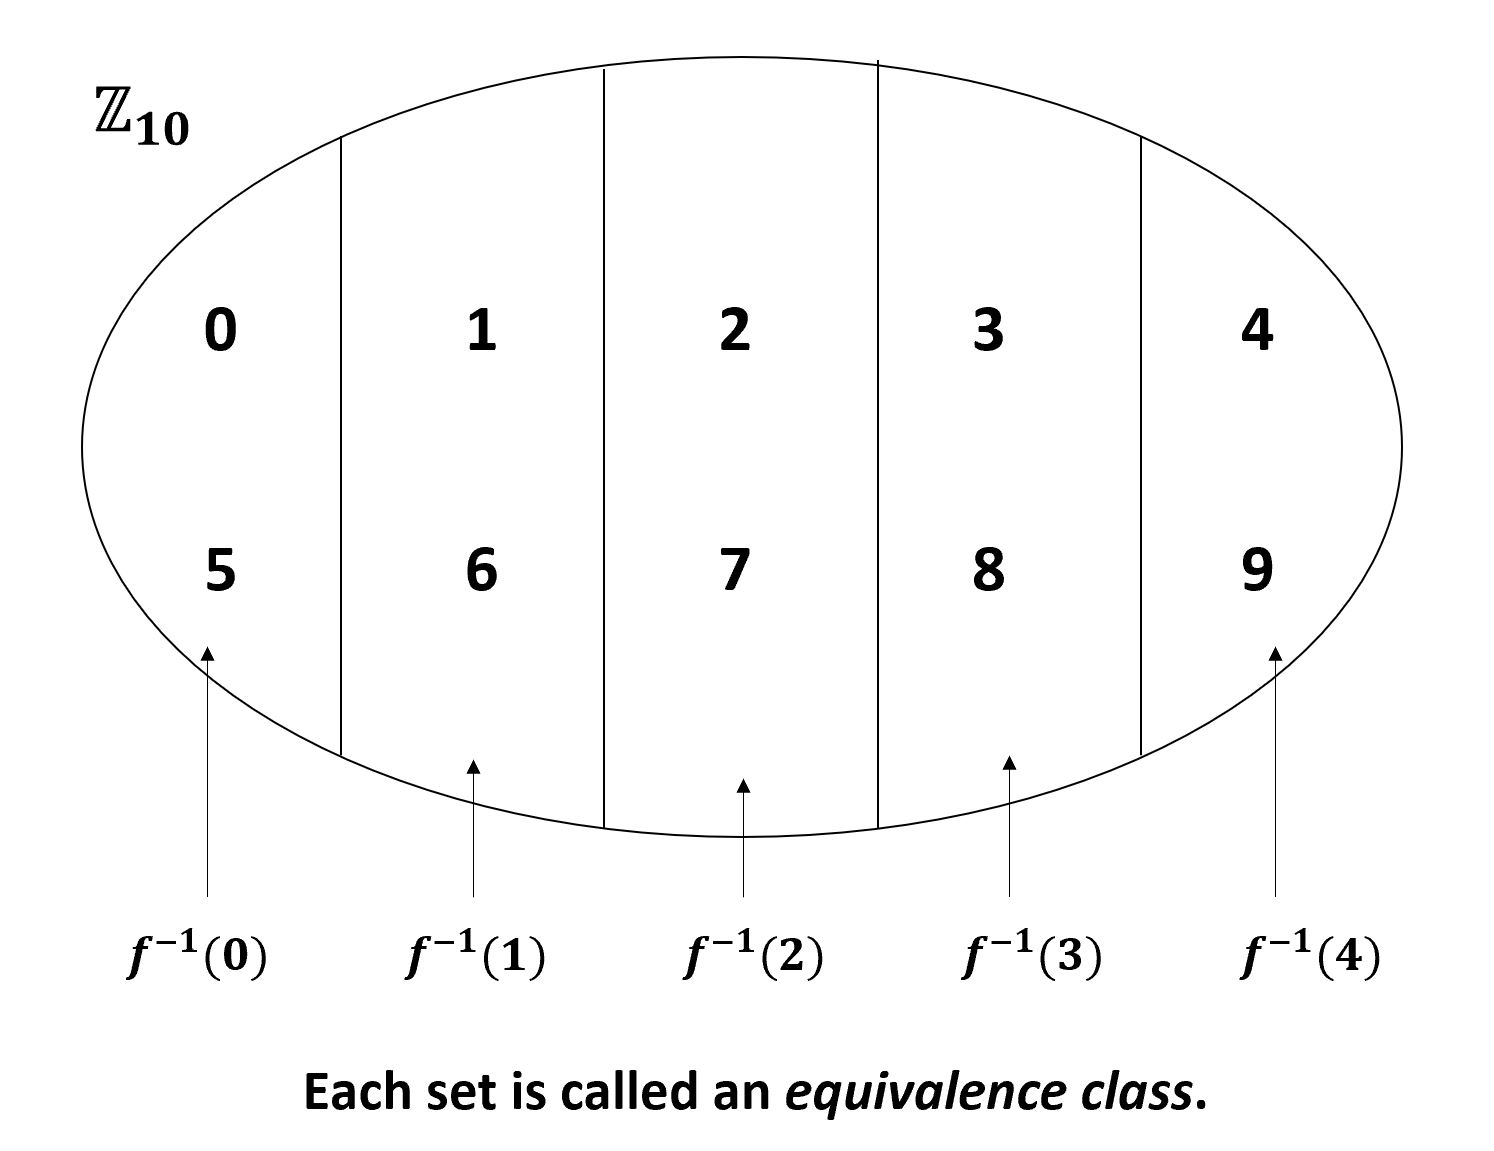
\includegraphics[width=3.5in]{images/Equivalence Class Image.jpg} }
\end{center}
\caption{Equivalence classes}\label{fig:equiv_class}
\end{figure}

We can create an addition and multiplication table on the equivalence classes. For example: $\{4,9\}+\{1,6\}$:
\begin{align*}
4+1&=5\\
9+1&=0\\
4+6&=0\\
9+6&=5
\end{align*}

Addition table:

\begin{center}
\begin{tabular}{c|c|c|c|c|c}
+ & $\{0,5\}$ & $\{1,6\}$ & $\{2,7\}$ & $\{3,8\}$ & $\{4,9\}$ \\
\hline
$\{0,5\}$ & $\{0,5\}$ & $\{1,6\}$ & $\{2,7\}$ & $\{3,8\}$ & $\{4,9\}$ \\
\hline
$\{1,6\}$ & $\{1,6\}$ & $\{2,7\}$ & $\{3,8\}$ & $\{4,9\}$ & $\{0,5\}$ \\
\hline
$\{2,7\}$ & $\{2,7\}$ & $\{3,8\}$ & $\{4,9\}$ & $\{0,5\}$ & $\{1,6\}$ \\
\hline
$\{3,8\}$ & $\{3,8\}$ & $\{4,9\}$ & $\{0,5\}$ & $\{1,6\}$ & $\{2,7\}$ \\
\hline
$\{4,9\}$ & $\{4,9\}$ & $\{0,5\}$ & $\{1,6\}$ & $\{2,7\}$ & $\{3,8\}$ 
\end{tabular}\\
\end{center}

Multiplication table:

\begin{center}
\begin{tabular}{c|c|c|c|c|c}
$\cdot$ & $\{0,5\}$ & $\{1,6\}$ & $\{2,7\}$ & $\{3,8\}$ & $\{4,9\}$ \\
\hline
$\{0,5\}$ & $\{0,5\}$ & $\{0,5\}$ & $\{0,5\}$ & $\{0,5\}$ & $\{0,5\}$ \\
\hline
$\{1,6\}$ & $\{0,5\}$ & $\{1,6\}$ & $\{2,7\}$ & $\{3,8\}$ & $\{4,9\}$ \\
\hline
$\{2,7\}$ & $\{0,5\}$ & $\{2,7\}$ & $\{4,9\}$ & $\{1,6\}$ & $\{3,8\}$ \\
\hline
$\{3,8\}$ & $\{0,5\}$ & $\{3,8\}$ & $\{1,6\}$ & $\{4,9\}$ & $\{2,7\}$ \\
\hline
$\{4,9\}$ & $\{0,5\}$ & $\{4,9\}$ & $\{3,8\}$ & $\{2,7\}$ & $\{1,6\}$ \\
\end{tabular}
\end{center}
\end{example}

The equivalence classes form a ring.  This is our first example of a \term{quotient ring}.  We write this ring as ${\mathbb Z}_{10}/{\mathbb Z}_5$.  (Recall we used a similar notation for quotient groups.)  We will formally define quotient rings below.

\begin{defn}\label{quotient ring}
Let $J$ be an ideal of ring $R$.  The \term{quotient ring} of $R$ by $D$ is the set $R/J$ consisting of all equivalence classes modulo $J$ in $R$, together with binary operations $+$ and $\cdot$ defined by the following:
\begin{align*}
(x+J)+(y+J)&=(x+y)+J \text{ and}\\
(x+J)\cdot(y+J)&=(x\cdot y)+J.
\end{align*}
\end{defn}

\begin{exercise}{Iso_Z10_to_Z5}
The quotient ring ${\mathbb Z}_{10}/{\mathbb Z}_5$ is isomorphic to another ring that we are familiar with. Can you identify this familiar ring?  \hyperref[ringsHints]{(*Hint*)} 
%answer: ${\mathbb Z}_5$
\end{exercise}

In the example above, we can say that ${\mathbb Z}_{10}/{\mathbb Z}_5$ is a quotient ring of ${\mathbb Z}_{10}$ by ${\mathbb Z}_5$ with four elements:
${\mathbb Z}_{10}/{\mathbb Z}_5=\{0+{\mathbb Z}_5, 1+{\mathbb Z}_5, 2+{\mathbb Z}_5, 3+{\mathbb Z}_5, 4+{\mathbb Z}_5\}$.

\begin{exercise}{Z3_homo}
Define $f:{\mathbb Z}_3\times {\mathbb Z}_3\rightarrow {\mathbb Z}_3$ by $f(a,b)=a$.
\begin{enumerate}[(a)]
\item Show that $f$ is a ring homomorphism.
\item What is the kernel of $f$?
\item What are the inverse images of $f$?
\item Use the definition of partition to show that the inverse images form a partition of the domain of $f$.
\item Make an addition and multiplication tables for the quotient ring, which consist of the inverse images.
\item What ring is isomorphic to the quotient ring?  \hyperref[ringsHints]{(*Hint*)} 
\end{enumerate}
\end{exercise}


\section{Integral domains, Principal ideal domains and fields}
\label{sec:IntegralDomainsPrincipalIdealDomains}

In high school algebra, we learn that if $a\cdot b=0$, then either $a=0$ or $b=0$.  This real number property is helpful when solving polynomial equations.  We will see that ring elements do not \emph{always} follow this rule.

\begin{defn}\label{zero_divisor}
If $a,b\in R$ with $a\neq 0,~b\neq 0,$ and $ab=0$, then $a$ and $b$ are called \term{zero divisors}.
\end{defn}

Before looking at general properties of zero divisors, let's look at some examples.

\begin{example}{Z21_zero_div}
In $Z_{21}$, $\{3,6,9,12,15,18,7,14\}$ are all zero divisors, since:
$3\cdot 7=6\cdot 7=9\cdot 7=12\cdot 7=15\cdot 7=18\cdot 7=14\cdot 3=0$.
\end{example}

\begin{exercise}{}
Find the zero divisors in ${\mathbb Z}_4$ and ${\mathbb Z}_{15}$.
\end{exercise}

In general, in ${\mathbb Z}_{p\cdot q}$, the elements $\{p,2p,\dots(q-1)p\}$ and $\{q,2q,\dots (p-1)q\}$ are all zero divisors.  

\begin{exercise}{}
Which of the following rings have zero divisors: $\mathbb{Z}$, $\mathbb{R}$, $\mathbb{C}$, and/or $\mathbb{Q}$?
\end{exercise}

The zero divisor property is closely related to invertibility, as shown in the following proposition.

\begin{prop}{zerodivisor}
Suppose that $R$ is a ring, and suppose $a \in R$ has a multiplicative inverse. Then $a$ is not a zero divisor--in other words, there is no $b \in R$ such that $b\neq 0$ and $a   b = 0$.
\end{prop}

\begin{exercise}{zerodivisor}
Prove Proposition~\ref{proposition:rings:zerodivisor}\hyperref[ringsHints]{(*Hint*)} 
\end{exercise}

Many rings have no zero divisors, other than zero itself.

\begin{defn}\label{int_dom}
A commutative ring that has no zero divisors is called an \term{integral domain}.
\end{defn}

${\mathbb Z},~{\mathbb R},~{\mathbb C},~and~{\mathbb Q}$ are all integral domains.

\begin{example}{integral_domain}
Show that ${\mathbb Z}_p$ is an integral domain if $p$ is prime.

\begin{proof}
We have shown in Example \ref{example:rings:Zn_ring} that ${\mathbb Z}_p$ is a commutative ring for all $p\in{\mathbb Z}$.  It remains to show that ${\mathbb Z}_p$ has no zero divisors.  We will show this by contradiction.

Suppose ${\mathbb Z}_p$ has a zero divisor $a\in{\mathbb Z}_p$ such that $a\neq 0$.  Then by Definition~\ref{zero_divisor}, there is some $b\in{\mathbb Z}_p$ such that $b\neq 0$ and $a\odot b=0$.  So:
\begin{align*}
&a\odot b=\bmod(ab,p)=0 & \text{Def. of }\odot\\
&p \text{ divides } ab & \text{Proposition }\ref{proposition:modular:equivalence_alt}\\
&p \text{ divides } a \text{ or } b & \text{Euclid's Lemma}\\
\end{align*}
But how can $p$ divide $a$ or $b$ when $p>a$ and $p>b$?  It is not possible.  So our assumption that ${\mathbb Z}_p$ has a zero divisor $a$ is false.  So ${\mathbb Z}_p$ has no zero divisors and ${\mathbb Z}_p$ is an integral domain.
\end{proof}
\end{example}

\begin{example}{}
Prove that ${\mathbb Q}[\sqrt[3]{2}]$ is an integral domain.

\begin{proof}
In Example \ref{example:rings:extension_ring} we showed that ${\mathbb Q}[\sqrt[3]{2}]$ is a ring.  It remains to show that ${\mathbb Q}[\sqrt[3]{2}]$ is commutative and contains no zero divisors.  We know that elements of ${\mathbb Q}[\sqrt[3]{2}]$ are real numbers, which are commutative by nature.  Thus, ${\mathbb Q}[\sqrt[3]{2}]$ inherits commutativity from the real numbers.  Additionally, real numbers have no zero divisors.  So again, this property is inherited by ${\mathbb Q}[\sqrt[3]{2}]$ and we can conclude that ${\mathbb Q}[\sqrt[3]{2}]$ is an integral domain.
\end{proof}
\end{example}

\begin{exercise}{}
Prove that  ${\mathbb Z}_n$ is an integral domain if and only if $n$ is prime.
\end{exercise}

\begin{exercise}{}
Let $R$ and $S$ be integral domains. Prove that $R\times S$ is also an integral domain.
\end{exercise}

\begin{exercise}{}
Prove or disprove:
\begin{enumerate}[(a)]
\item
The ring $M_2(R)$ is an integral domain.
\item
The subring of $M_2(R)$ consisting of diagonal matrices is an integral domain. (By ``diagonal matrix'' we mean matrices of the form 
$ \begin{bmatrix}
a & 0 \\ 0 & b
\end{bmatrix}$).
\item
The subring of $M_2(R)$ consisting of upper triangular matrices is an integral domain. (Upper triangular matrices have the form 
$ \begin{bmatrix}
a & b \\ 0 & c
\end{bmatrix}$).
\end{enumerate}
\end{exercise}

An important property of integral domain is the cancellation law of multiplication, as shown in the following proposition.

\begin{prop}{cancellation_law}
Given integral domain $D$ and $a,b,c\in D$.  If $ab=ac$ and $a\neq 0$, then $b=c$.

\begin{proof}
\begin{align*}
    ab&=ac & \text{Given}\\
    ab-ac&=0 & \text{Substitution}\\
    a(b-c)&=0 & \text{Distributive Law}\\
\end{align*}
Since $D$ is an integral domain, then $D$ has no zero divisors.  This means that $a=0$ or $b-c=0$.  But we know that $a\neq 0$.  So $b-c=0$ and $b=c$.
\end{proof}
\end{prop}


In Definition \ref{principal_ideal} we learned that a principal ideal is generated by a single element of a ring, $R$.  We can now combine this idea with that of the integral domain.

\begin{defn}\label{princ_ideal_dom}
A \term{principal ideal domain} is an integral domain, all of whose ideals are principal.
\end{defn}

It turns out that ${\mathbb Z},~{\mathbb R},~{\mathbb C},~{\mathbb Q},~{\mathbb Z}_p,~{\mathbb R}[x],~{\mathbb C}[x],~{\mathbb Q}[x]$, and ${\mathbb Z}_p[x]$ are all principal ideal domains.  Unfortunately, we are not prepared to prove this here.\footnote{The proof that ${\mathbb Z}$ is a principal ideal domain makes use of the \term{well-ordering principle} which states that any subset of ${\mathbb N}$ has a smallest element.  The interested reader may consult \url{https://faculty.atu.edu/mfinan/4033/abstractbk.pdf} (p. 219) for more details.}\\

Let's explore another important ring subset known as the \emph{prime ideal}.  We shall see that the concept of prime ideal is closely related to prime numbers.


\begin{example}{not_prime_ideal}
Suppose we are given the set $J\subset{\mathbb Z}:J=\{\cdots,-12,-6,0,6,12,\cdots\}$.  Prove or disprove that $p,q\in{\mathbb Z}$ and $p\cdot q\in J$ implies $p\in J$ or $q\in J$. 
\end{example}

\begin{proof}
We can disprove this by counterexample.  Consider, for example, $3,4\in{\mathbb Z}$.  It is true that $3\cdot 4=12\in J$, but neither $3$ nor $4$ is in $J$.  (Many other counterexamples can be found.)
\end{proof}

\begin{exercise}{prime_ideals}
\begin{enumerate}[(a)]
\item Suppose $J=\{\cdots,-14,-7,0,7,14,\cdots\}$ in the example above.  Prove or disprove that $p,q\in{\mathbb Z}$ and $p\cdot q\in J$ implies $p\in J$ or $q\in J$.
\item Suppose $J=\{\cdots,-2a,-a,0,a,2a,\cdots\}$ for some $a\in{\mathbb Z}$ and $p,q\in{\mathbb Z}$.  For what values of $a$ is it true that $p\cdot q\in J$ implies $p\in J$ or $q\in J$? 
\end{enumerate}
\end{exercise}

The previous exercise is an example of a \emph{prime ideal}, defined below. 

\begin{defn}\label{prime_ideal}
A \term{prime ideal} $J\subset R$ is an ideal such that if $p,q\in R$ and $p\cdot q\in J$, then either $p\in J$ or $q\in J$.
\end{defn}

\begin{defn}\label{prime element}
When a principal ideal $Ra$ is also a prime ideal, then the generator $a$ is called a \term{prime element}
\end{defn}

In Exercise \ref{exercise:rings:prime_ideals} (a) you showed that $7$ is a prime element.  However, the result of (b) implies that $7^n$ where $n>1$ is \emph{not} a prime element.  The following definition applies to powers of prime elements.

\begin{defn}\label{prime_power_ideal}
Suppose $a$ is a prime element in the ring $R$.  Then for any positive integer $n$, $a^n$ is called a \term{prime power} and $R(a^n)$ is called a \term{prime power ideal}.
\end{defn}

We will explore these concept in the next exercise.

\begin{exercise}{}
\begin{enumerate}[(a)]
\item In the ring of integers, show that $2{\mathbb Z}$ is a prime ideal.
\item In the ring of integers, show that $8{\mathbb Z}$ is \emph{not} a prime ideal, but it is a prime power ideal.
\end{enumerate}
\end{exercise}

We will conclude this section with an important result in abstract algebra that closely resembles prime factorization of integers.

\begin{prop}{int_PPI}
In a principal ideal domain, any principal ideal is the intersection of prime power ideals.\\
\end{prop}

\begin{proof}
This is a more difficult proof and will not be studied in this class.
\end{proof}

In the following example, we will see that all principal ideals factor as an intersection of prime power ideals.

\begin{example}{}
Show that $12{\mathbb Z}=2^2{\mathbb Z}\cap 3{\mathbb Z}$.
\end{example}

\begin{proof}
Recall that:
\begin{align*}
&12{\mathbb Z}=\{12n:n\in{\mathbb Z}\}=\{\cdots,-24,-12,0,12,24,\cdots\},\\
&2^2{\mathbb Z}=4{\mathbb Z}=\{4n:n\in{\mathbb Z}\}=\{\cdots,-8,-4,0,4,8,\cdots\}, \text{ and}\\ &3{\mathbb Z}=\{3n:n\in{\mathbb Z}\}=\{\cdots,-6,-3,0,3,6,\cdots\}.  
\end{align*}
Since $4$ and $3$ are relatively prime, then the only common multiples of $4$ and $3$ will be multiples of $4\cdot 3$ or $12$.  In other words, $2^2{\mathbb Z}\cap 3{\mathbb Z}=4{\mathbb Z}\cap 3{\mathbb Z}=(4\cdot 3){\mathbb Z}=12{\mathbb Z}$.
\end{proof}

\begin{exercise}{}
Show that $42{\mathbb Z}=2{\mathbb Z}\cap 3{\mathbb Z}\cap 7{\mathbb Z}$.
\end{exercise}

Proposition \ref{proposition:rings:int_PPI} is the algebraic way of proving that any integer is the product of primes. The proposition also shows that polynomial can be factored uniquely.  We will explore this more in Section~\ref{sec:polyOverFields} when we discuss polynomial rings.  We need a bit more ring theory first.

\subsection{Division rings and fields\quad
\sectionvideohref{Q5q-LL4QW4o&list=PL2uooHqQ6T7PW5na4EX8rQX2WvBBdM8Qo&index=48}}


%%%% We want to start talking about rings that have a multiplicative identity and inverses.  We'll need some terminology for this. So let's kick off with a definition:

%%%% \begin{defn}
%%%% A \term{ring with unit} is a ring that has a multiplicative identity (the multiplicative identity is usually denoted as 1).
%%%% \end{defn}

%%%% \begin{exercise}{}
%%%% Give an example of (a) a ring with unit, and (b) a ring without unit. Explain your answers.
%%%% \end{exercise}
%A possible solution is $nZ$, where $n\eq 1$. $nZ= {...,-3n, -2n, -n, 0, n, 2n, 3n, ...}$. Notice the multiplicative identity for $nZ$, $1$, is not included int he set.
All of the rings we have seen so far have multiplicative identities. But it is impossible to define multiplicative inverses for all the elements. In fact, it's (almost) \emph{never} possible to  have a multiplicative inverse of the additive identity (which we denote as 0), as long as the distributive property holds.

\begin{exercise}{}
There is one and only one case of a ring $R$ in which every element has a multiplicative inverse. What is $R$? 
\end{exercise}

\begin{exercise}{}
Suppose the ring $R$ has more than one element.  Show that the additive identity of $R$ has no multiplicative inverse.
\end{exercise}

%%%% \begin{exercise}{noInvFor0}
%%%% \begin{enumerate}[(a)]
%%%% \item
%%%% Let $R$ be a ring, and let $0$ be the additive identity of $R$.  Show that $a \cdot 0 = 0 \cdot a = 0$ for any element $a \in R$. 
%%%% \hyperref[sec:polyrings:hints]{(*Hint*)} 
%%%% \item
%%%% Part (a) shows that every ring element times 0 must be equal to 0.  So in order for 0 to have an inverse, 0 must also be the multiplicative identity. Show that 
%%% if $R$ has two or more elements, then 0 cannot be the multiplicative identity of $R$.
%%%% \item

%%%% \end{enumerate}
%%%% \end{exercise} 

%\begin{enumerate}[{a}]
% \item
%Let $ a, b \in R$ be arbitrary.
%
%Now $a\cdot(b+0)=a\cdot b+a\cdot 0$, because left distributivity holds for rings. 
%On the other hand, $a\cdot(b+0)=a\cdot b$,  because $0$ is the additive identity.
%By substitution,   
%$$a \cdot b+a\cdot 0=a\cdot b.$$
%Adding $-(a\cdot b)$ to both sides, we obtain
%$$a\cdot 0=0$$.
%We may use a similar argument using $(b+0)\cdot a$ instead of $a \cdot (b+0)$ to show that 
%$0\cdot a = 0$.
%\end {proof}

%\item 
%We may use proof by contradiction. Since $R$ has at least two elements, $R$ must have an element that is not 0. Call it $a$. Suppose that $0$ is the multiplicative identity in $R$. Then $a\cdot 0=a$. However, by part (a) we have $a\cdot 0=0$. By substitution, this would imply $a=0$, which contradicts our assumption. 
%\end{enumerate}

Although the zero element never has a multiplicative inverse, there are cases where multiplicative inverses exist for every \emph{nonzero} element of a ring. Such a ring is called a \emph{division ring}. 

\begin{defn} \label{def:divisionring}
Given a ring $R$ suppose every nonzero element of $R$ has a multiplicative inverse in $R$, then $R$ is called a \term{division ring}.
\end{defn}

Let's explore an important example of division rings.  In Example \ref{example:groups:quaternions} we introduced a special group called the quaternion group,\\ $Q_8=\{1,-1,i,-i,j,-j,k,-k\}$, with the following relations:
\begin{enumerate}[(a)]
\item
$1$ is the identity
\item
$-1$ commutes with all other elements, and $(-1)^2=1$
\item
$-1 \cdot i = -i, -1 \cdot j = -j, -1 \cdot k = -k$
\item
$i^2 = j^2=k^2 = -1$
\item
$i \cdot j = k, j \cdot k = i, k \cdot i=j$
\item
$j \cdot i = -k, k \cdot j=-i, i \cdot k = -j$ 
\end{enumerate}

% Properties (d),(e),(f) can be summarized as follows:
% \begin{equation}\label{quat}
% i^2=j^2=k^2=ijk=-1.
% \end{equation}

\begin{exercise}{}
Show that all of the equalities in parts (e) and (f) above may be derived from (a), (b), (c) and the equation $ijk=-1$. 
\end{exercise}

We can extend the quaternion group by taking linear combinations of the elements of ${\mathbb Q}_8$ with real coefficients.  This new set, simply known as the \emph{quaternions}, was discovered by William Rowan Hamilton of Dublin in 1843.  Hamilton's quaternions, notated by ${\mathbb H}$ in his honor, are widely used today in computer graphics to describe motion in three dimensional space and multiple antennae communications systems.  We may define this set formally as follows.

\begin{defn}\label{quaternionring}
The set of real \term{quaternions}, denoted by ${\mathbb H}$, is defined by:
\begin{center}
${\mathbb H}=\{a_0+a_1i+a_2j+a_3k:a_0,a_1,a_2,a_3\in {\mathbb R}\}$,

where $i^2=j^2=k^2=ijk=-1$.
\end{center}

Note that $ij=-ji$, $ik=-ki$, and $jk=-kj$, so ${\mathbb H}$ does \emph{not} commute over multiplication.

Using the distributive law and the commutative law of addition, we define addition on ${\mathbb H}$ as follows.
\begin{equation}
\begin{aligned}
&(a_0+a_1i+a_2j+a_3k)+(b_0+b_1i+b_2j+b_3k)\\
&=(a_0+b_0)+(a_1+b_1)i+(a_2+b_2)j+(a_3+b_3)k.
\end{aligned}
\end{equation}
Multiplication of quaternions is also defined using the distributive law and commutative law of addition.
\end{defn}

\begin{exercise}{}
Evaluate the following products of quaternions.
\begin{enumerate}[(a)]
\item $(1+i+j+k)^2$
\item $(1+i+j+k)\cdot (1-i-j-k)$
\item $(1+i+j+k) \cdot (1+2i+3j+4k)$
\item $(a_0+a_1i+a_2j+a_3k)\cdot (a_0-a_1i-a_2j-a_3k)$
\end{enumerate}
\end{exercise}


In the following exercises, we will show that ${\mathbb H}$ forms a division ring.

\begin{exercise}{}
Prove that the set of quaternions ${\mathbb H}$, defined above, forms a ring.
\end{exercise}

Of course, not all rings are division rings.  In order to show that ${\mathbb H}$ is a division ring, we must show that every nonzero element of ${\mathbb H}$ has a multiplicative inverse in ${\mathbb H}$.  This proof is more advanced so you will be guided through it.  

We will begin by defining the \emph{conjugates} in ${\mathbb H}$.  (Note that the term \emph{conjugates}, like many other mathematical terms, can refer to different things in different contexts.  The reader must always consider context to fully understand the meaning of such terms.)

\begin{defn}
Let $a=a_0+a_1i+a_2j+a_3k\in{\mathbb H}$.  Then the \term{conjugate} of $a$ is denoted by $\bar{a}$ and given by:
\begin{center}
$\bar{a}=a_0-a_1i-a_2j-a_3k$.
\end{center}
\end{defn}

Note the following relationship between $a$ and $\bar{a}$:
\begin{align*}
a\cdot \bar{a}&=(a_0\cdot a_0+a_1\cdot a_1+a_2\cdot a_2+a_3\cdot a_3)+(-a_0\cdot a_1+a_0\cdot a_1-a_2\cdot a_3+a_2\cdot a_3)i\\
&+(-a_0\cdot a_2+a_0\cdot a_2-a_1\cdot a_3+a_1\cdot a_3)j+(-a_0\cdot a_3+a_0\cdot a_3-a_1\cdot a_2+a_1\cdot a_2)k\\
&=a_0\cdot a_0+a_1\cdot a_1+a_2\cdot a_2+a_3\cdot a_3\\
&=a_0^2+a_1^2+a_2^2+a_3^2
\end{align*}

\begin{exercise}{}
\begin{enumerate}[(a)]
\item Using $a$ and $\bar{a}$ as defined above, show that $\bar{a}\cdot a=a\cdot\bar{a}$.
\item Note that if $a\neq 0$, $a\cdot \bar{a}$ is a nonzero real number and thus has a multiplicative inverse $(a\cdot \bar{a})^{-1} $. Show that $a\cdot\left( (a\cdot \bar{a})^{-1}\cdot \bar{a}\right)=1$ and $\left( (a\cdot \bar{a})^{-1}\cdot \bar{a}\right)\cdot a=1$.
\item Give an expression for the multiplicative inverse of $a\in{\mathbb H}$ for $a\neq 0$.
\end{enumerate}
\end{exercise}

We have shown that the set of quaternions ${\mathbb H}$ is a ring and that every nonzero element of ${\mathbb H}$ has a multiplicative inverse in ${\mathbb H}$.  So, ${\mathbb H}$ is a division ring.


\begin{exercise}{}
\begin{enumerate}[(a)]
\item
Give three examples of infinite division rings.
\item
Give three examples of finite division rings.
\end{enumerate}
\end{exercise}
%The following infinite rings are division rings because all nonzero elements have multiplicative inverses: $\mathbb{Q}$,  $\mathbb{R}$,  and $\mathbb{C}$. Similarly $\mathbb{Z}_3$, $\mathbb{Z}_5$, and $\mathbb{Z}_7$ are all finite division rings, since each nonzero element has a multiplicative inverse (Proposition 3.5.28). 

Division rings with commutative multiplication are called \term*{fields}.  Fields are one of the most important objects of study in all of mathematics.

\begin{defn} \label{def:field}
A division ring $F$ is called a \term{field} if the multiplication operation is commutative. \end{defn}

In many of the rings we've seen so far, the field axioms are also satisfied.  Figure \ref{fig:ring_classes} shows the relationship between the ring classes.

\begin{figure}[H]
%\begin{center}
\centerline {
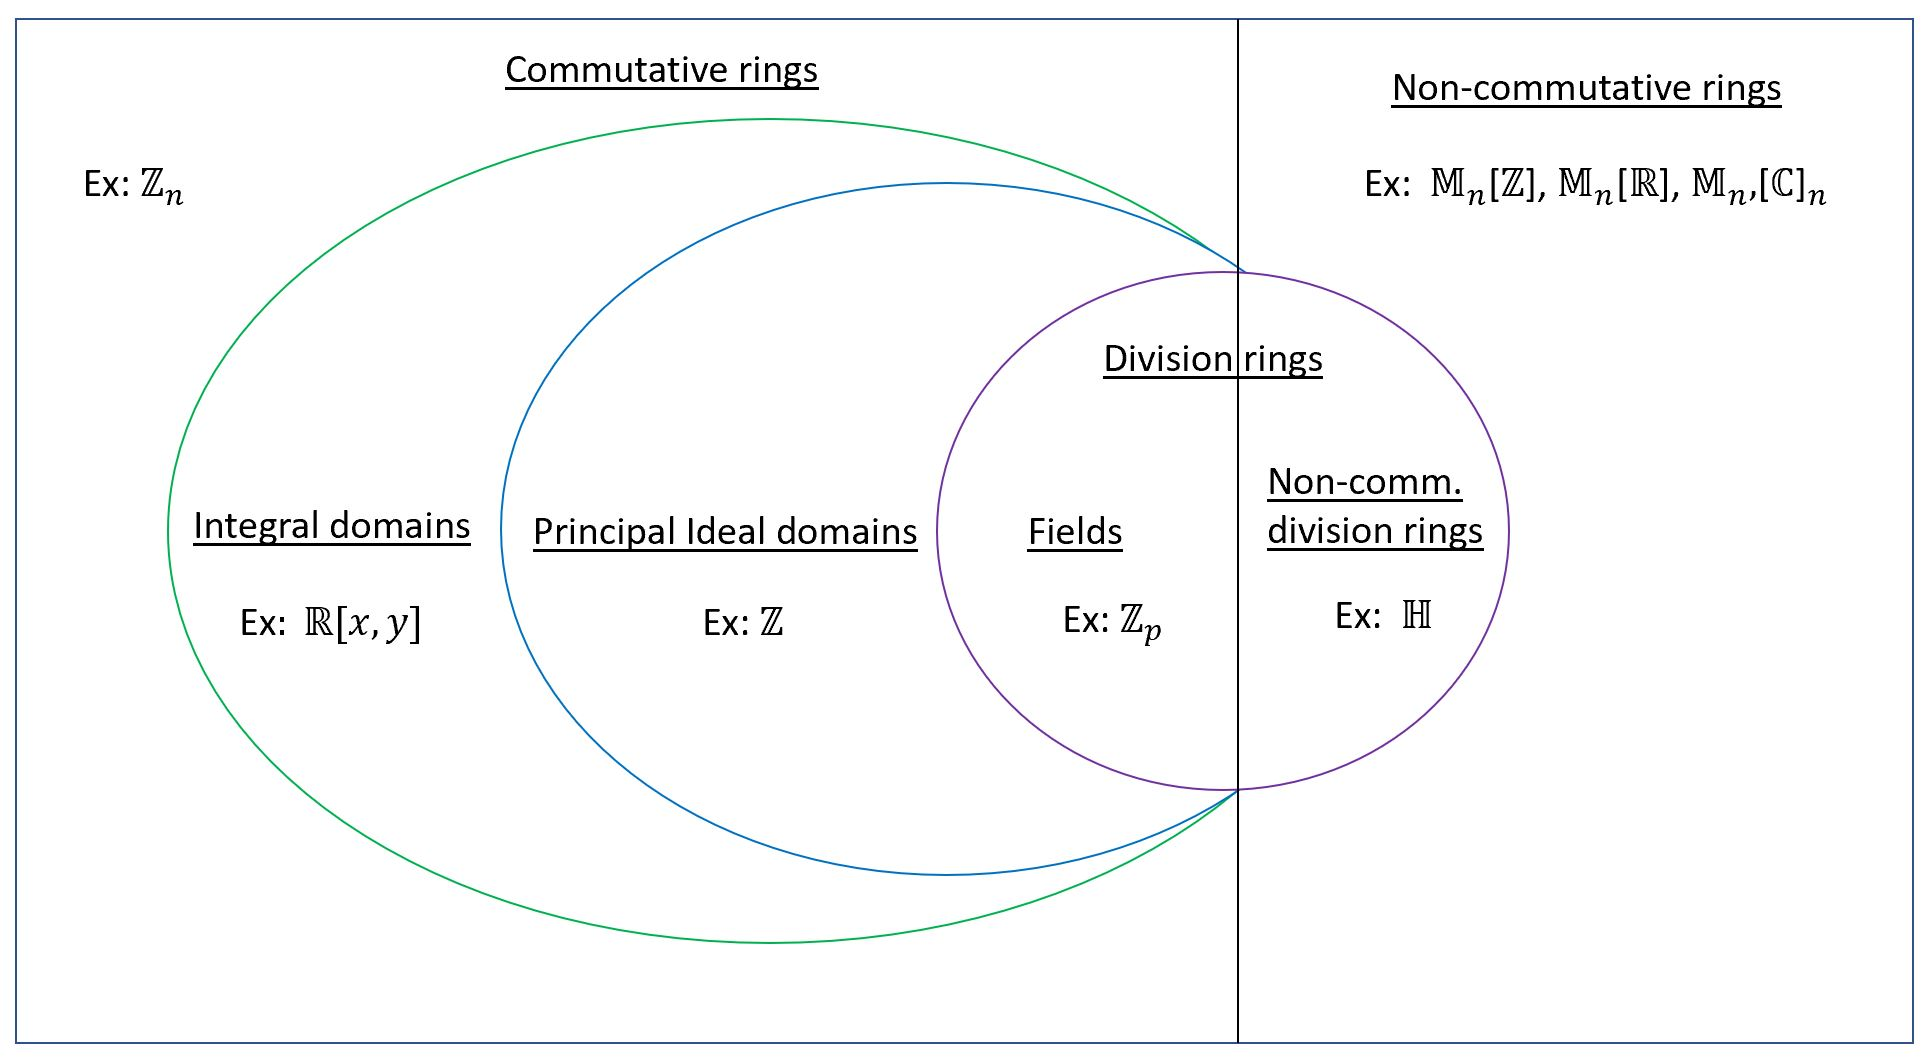
\includegraphics[width=5.5in]{images/RingClasses.jpg} }
%\end{center}
\caption{Ring Classes}\label{fig:ring_classes}
\end{figure}
%%%% In the following discussion, we will be considering the case where the polynomial coefficients form a field. We will see in Section~\ref{divisionalgorithm} that this allows us to perform polynomial long division and determine gcd's, very much like we did with integers in the modular arithmetic chapter.

\begin{exercise}{poly47}
Which of the following rings are also fields?  Explain your answers.

(a) ${\mathbb Z}$\quad
(b) ${\mathbb Q}$\quad
(c) ${\mathbb R}$\quad
(d) ${\mathbb C}$\quad
(e) ${\mathbb R}[x]$\quad  
(f) ${\mathbb M}_n({\mathbb R})$\quad
(g) $3{\mathbb Z}$\quad
(h) ${\mathbb Z}_4$\quad

(i) ${\mathbb Z}_p$ where $p$ is prime
\end{exercise}

\begin{example}{}
Let $S$ be the set of all real $2\times 2$ matrices of the form $\begin{bmatrix}
a & b\\
-b & a 
\end{bmatrix}$
where $a,b\in{\mathbb R}$.  Show that $S$ is a field.

\begin{proof}
We know from Exercise \ref{exercise:rings:ringMatrices} that the set of all $2\times 2$ matrices form a ring.  It remains to show that $S$ is a division ring with multiplicative commutativity.  It will be important in our proof to know that $S$ has the multiplicative inverse property.  Let's show that first.

Let $A\in S$ be defined by
$\begin{bmatrix}
a & b\\
-b & a
\end{bmatrix}.$
Then $A^{-1}=
\begin{bmatrix}
\frac{a}{a^2+b^2} & -\frac{b}{a^2+b^2}\\
\frac{b}{a^2+b^2} & \frac{a}{a^2+b^2}
\end{bmatrix}$ (as long as $a$ and $b$ are not both 0)
because $A\cdot A^{-1}=A^{-1}\cdot A=1$.  It should be clear that $A^{-1}\in S$.  Thus every nonzero element of $S$ has an inverse in $S$ and the multiplicative inverse property holds.  We are now ready to show that $S$ is a division ring.

We will show that $S$ is a division ring by showing that it has no zero divisors.  At this point, Proposition~\ref{proposition:rings:zerodivisor} comes in handy.  We've already seen that every nonzero element  $A \in S$ has an inverse. Proposition~\ref{proposition:rings:zerodivisor} immediately tells us that $A$ is not a zero divisor. Since $A$ was an arbitrary element of $S$, then there are no zero divisors in $S$ and $S$ is a division ring.
  
We have shown that $S$ is a division ring, but we must now prove commutativity of multiplication.

Given $X=
\begin{bmatrix}
a & b\\
-b & a
\end{bmatrix}$
and $Y=
\begin{bmatrix}
c & d\\
-d & c
\end{bmatrix}
\in S$, then: 

$X\cdot Y=
\begin{bmatrix}
ac-bd & ad+bc\\
-ad-bc & ac-bd
\end{bmatrix}$
and $Y\cdot X=
\begin{bmatrix}
ac-bd & ad+bc\\
-ad-bc & ac-bd
\end{bmatrix}. $

We have shown that $X\cdot Y=Y\cdot X$ for any $X,Y\in S$, so $S$ is commutative over multiplication.  So $S$ is a division ring with commutativity of multiplication, which means $S$ is a field.
\end{proof}
\end{example}

\begin{exercise}{}
Show that the set of matrices $S=
\begin{bmatrix}
a & b\\ 
0 & a 
\end{bmatrix}$
where $a,b\in {\mathbb R}$ is \emph{not} a field.
\end{exercise}

Looking bac at Section~\ref{sec:extensionRings} we can see that we were creating fields without knowing it!  The sets $\widehat{\mathbb{Q}}[x]$, 
$\widehat{\mathbb{R}}[x]$,
$\widehat{\mathbb{Z}}_p[x]$,
$\widehat{\mathbb{C}}[x]$
are all fields that are extensions of $\mathbb{Q}[x]$, 
$\mathbb{R}[x]$,
$\mathbb{Z}_p[x]$,
$\mathbb{C}[x]$. 

\subsection{Further properties of fields}

We've just introduced several new concepts, including integral domain, principal ideal domain, division ring, and field. Let's consider how they are related. We know that every field is a division ring (by definition). We also know that not every division ring is a integral domain (${\mathbb H}$ is a example). What about the relation between integral domain and field?

\begin{exercise}{field_is_ID}
Show that every field is an integral domain. 
\end{exercise}

Now, what about the relation between field and principal ideal domain? This is  a very interesting question. To answer it, we will need a series of propositions.

\begin{prop}{1inIdeal}
If $J$ is an ideal of the ring $R$ and $1 \in J$, then $J = R$.
\end{prop}

\begin{exercise}{1inIdeal}
Prove Proposition~\ref{proposition:rings:1inIdeal}
\end{exercise}


%%% Definition \ref{def:ideal}

%Note that in general, a ring does not require the properties of commutativity, multiplicative inverse or multiplicative identity.  Rings that satisfy these additional conditions form a field.

\begin{prop}{idealWithInv}
Given $J$ is an ideal in ring $R$ and $a\in J$.  If $a$ has a multiplicative inverse $a^{-1}\in R$, then $J=R$.
\end{prop}

\begin{proof}{}
To show that $J=R$, we can show that $J\subset R$ and $R\subset J$.  We already know that $J\subset R$, by definition of ideal.  To show that $R\subset J$, we must show that every element in $R$ is also in $J$.  Consider arbitrary element $r\in R$. We will show that $r\in J$ also.

\begin{align*}
 &a\in J \text{ implies } a^{-1}\in R & \text{Given}\\
 &a\cdot a^{-1} = 1 & \text{Def. of mult. inverse}\\
 &a\in J \text{ and } a^{-1}\in R \text{ implies } a\cdot a^{-1}=1\in J & \text{Def. of ideal}\\
 &J = R  & \text{Proposition~\ref{proposition:rings:1inIdeal}}
\end{align*}

\end{proof}


\begin{prop}{}
Given field $F$, the only two ideals in $F$ are $\{0\}$ and all of $F$.

\begin{proof}
Suppose $J$ is an ideal in field $F$.  Then either $J=\{0\}$ or $J$ has a nonzero element $a$. By the definition of field, $a$ must have an inverse; and by Proposition~\ref{proposition:rings:idealWithInv}, it follows that $J=F$.
\end{proof}
\end{prop}

We've also discussed principal ideal domain which is a special type of integral domain.

\begin{exercise}{}
What is the relationship between fields and principal ideal domains?
\end{exercise}

See if you can prove this final proposition that relates the ideas of field and ideal. 

\begin{prop}{idealField}
Suppose that $R$ is a commutative ring such that every ideal contains the multiplicative identity 1. Then every element in $R$ has a multiplicative inverse. In other words, $R$ is a field.\\
\end{prop}

\begin{exercise}{idealField}
Prove Proposition~\ref{proposition:rings:idealField}
\end{exercise}


\section{Polynomials over fields}
\label{sec:polyOverFields}

We saw in the previous section that  $R[x]$ is a ring whenever $R$ is a ring. We may ask a similar question about fields: If $F$ is a field, then is $F[x]$ also a field? We investigate this question in the following exercises.


\begin{exercise}{poly12}
\begin{enumerate}[(a)]
\item  Give the zero divisors of ${\mathbb Z}_4$ and ${\mathbb Z}_{15}$.
\item
Find two nonzero polynomials in $\mathbb{Z}_4[x]$ of degree 1 and 3 respectively  whose product is 0.
\item
Suppose $n=pq$, where $p$ and $q$ are integers greater than 1. Show that there exist two nonzero polynomials in $\mathbb{Z}_n[x]$ with degree greater than 1 whose product is 0.
\end{enumerate}
\end{exercise}
%Solution
%\begin{enumerate}[(a)]
%\item 
%Let $p(x)=2x^3$ and $q(x)=2x$. Then, $p(x)\cdot q(x)=2x^3\cdot 2x = (2\cdot2)x^4=0x^4=0$.
%\item
%Let $pq=n$. This implies that $p<n$ and $q<n$. Therefore $p\in Z_n$ and $q\in Z_n$. Now,$p(x)\cdot q(x)=(p\cdot q)x=0x$, since $pq=n$.
%\end{enumerate}

Do polynomials have multiplicative inverses? Be careful here. In high-school algebra or in calculus,   the polynomial $p(x)$ has a perfectly good multiplicative inverse, namely  $1/p(x)$. But $1/p(x)$ is not a polynomial, so for us it doesn't count! For a set of polynomials to be a field, the nonzero elements must have inverses that are polynomials themselves.

\begin{exercise}{}
\begin{enumerate}[(a)]
\item
Consider the  polynomial $p(x)= 1x$ as an element of $\mathbb{R}[x]$. Show there is no polynomial in $\mathbb{R}[x]$ that is a multiplicative inverse of $p(x)$.
\item
Prove or disprove: Polynomial rings over fields are also commutative groups over multiplication.
\end{enumerate}
\end{exercise}

\begin{exercise}{}
Which elements of $\mathbb{R}[x]$ have multiplicative inverses?
\end{exercise}


\begin{exercise}{}
Given a field $F$, which elements of $F[x]$ have multiplicative inverses?
\end{exercise}

\begin{exercise}{fieldexercise}
Suppose that $F$ is a field. Does this mean that $F[x]$ is also a field? Either prove the implication, or give a counterexample.
\end{exercise}

We may ask the question, Can $F[x]$ have zero divisors if $F$ is a field? First let's look at an example.

\begin{exercise}{zdzp}
Let $p(x)=\sum_{i=0}^{5} a_ix^i$ and $q(x)=\sum_{j=0}^{3} b_jx^j$ be polynomials in $\mathbb{Z}_p[x]$, where $a_5\neq 0$ and $b_3\neq 0$.
\begin{enumerate}[(a)]
\item
What is the degree of $p(x)q(x)$?
\item
Give an expression for the highest order term in $p(x)q(x)$. How do you know that this expression is not zero? \hyperref[ringsHints]{(*Hint*)} 
\end{enumerate}
Note that since $p(x)q(x)$ has a nonzero term, then it can't be the zero polynomial.
\end{exercise}

\noindent
We may generalize the results of the previous exercise:

\begin{exercise}{zdzp}
Let $p(x)=\sum_{i=0}^{n} a_ix^i$ and $q(x)=\sum_{j=0}^{m} b_jx^j$ be polynomials in $F[x]$, where $F$ is a field and $a_n\neq 0$, $b_m\neq 0$.
\begin{enumerate}[(a)]
\item
What is the degree of $p(x)q(x)$?
\item
Give an expression for the highest order term in $p(x)q(x)$. How do you know that this expression is not zero? 
\end{enumerate}
\end{exercise}

Exercise \ref{exercise:rings:zdzp} establishes the following proposition: 

\begin{prop}{nozerodiv} If $F$ is a field, then $F[x]$ has no zero divisors.
\end{prop}

The property of having no zero divisors turns out to be a very important consideration in the process of polynomial division, which we discuss in the next section.

And here's the result we've been waiting for. Now that we've prepared the ground, it's not so difficult to prove.

\begin{prop}{FTOA}(\emph{Fundamental Theorem of Algebra: easy part})
Let $F$ be a field and let $f(x)$ be a polynomial in $F[x]$ of degree $n$. Then the equation $f(x)=0$ has at most $n$ solutions: that is, there are at most $n$ distinct elements $\{x_1,\ldots x_n\}$ of $F$ such that $f(x_m)=0$ for $1 \le m \le n$.
\end {prop}


\begin{proof}
Suppose $a_1$ is a solution to $f(x)=0$. Then by Proposition~\ref{proposition:poly:polydivides} it follows that $x-a_1$ divides $f(x)$. Therefore $f(x) = (x-a_1) g_{n-1}(x)$ where the degree of $g_{n-1}(x)=n-1$. 

Now if $a_2 \neq a_1$ is another solution then using our above result we have
\[ f(a_2) = (a_2 - a_1)g_{n-1}(a_2) = 0. \]
Since $a_2 - a_1 \neq 0$, it follows that $g_{n-1}(a_2) = 0$. So we can write $g_{n - 1}(x) = (x-a_2)g_{n-2}(x)$ where the degree of $g_2(x) = n-2$. 

Continuing in the same way, if there are distinct roots $a_1,a_2,...,a_n$ then 
\[
f(x) = (x - a_1)(x - a_2)...(x - a_n)g_0, \]
 where the degree of $g_0$ is 0 (in other words, $g_0$ is a constant.). So there can't be any more solutions, $a_{n+1}$, because $(x-a_{n+1})$ doesn't divide $g_0$.
\end {proof}

The previous theorem immediately gives us an extremely important general property of fields:

\begin{prop}{atmostnroots}
Let $F$ be a field, and let $c$ be any element $F$.  Then $c$ has at most $n$ $n^{\text{th}}$ roots.
\end {prop}


\begin{proof}
Given the field $F$ let $F[x]$ be the associated polynomial ring over the field $F$. The polynomial $x^n-c$ is an element of $F[x]$. By Proposition~\ref{proposition:rings:FTOA}, the equation $x^n-c=0$ has at most $n$ solutions.  This is exactly the same thing as saying that $c$ has at most $n$ $n^{\text{th}}$ roots.
\end {proof}

\begin{exercise}{roots}
\begin {enumerate}[(a)]
\item
Find all fourth roots of 5625 in $\mathbb{R}[x]$. Give exact solutions.
\item
Find all fifth roots of $3125i$ in $\mathbb{C}[x]$. Give exact solutions. 
\item
Find all fifth roots of 5 in $\mathbb{Z}_7$.
\item
Find all sixth roots of 1 in $\mathbb{Z}_7$.
\end{enumerate}
\end{exercise}


Take note of the ``at most'' qualification in Proposition~\ref{proposition:rings:FTOA}. There are cases of polynomials in $F[x]$ which do not have  \emph{any} roots in $F$. For example, there are polynomials in $\mathbb{R}[x]$ that have no roots at all in $\mathbb{R}[x]$, as the next examples illustrate.

\begin{example}{poly_complex} 
Find the roots of $p(x)=2x^2+2x+5$.

Since this is a quadratic polynomial we can use the famous quadratic formula:

$$x=\frac {-b \pm \sqrt{b^2-4ac}}{2a}$$

In $p(x), a=2, b=2$, and $c=5.$ We substitute those values into the formula and obtain the following:
\begin{align*}
x&=\frac {-2 \pm \sqrt{2^2-4\cdot 2\cdot 5}}{2\cdot 2}=\frac {-2 \pm \sqrt{-36}}{4}=\frac {-2 \pm 6i}{4}\\
&=\frac {-1 \pm 3i}{2}.
\end{align*}

So the roots of $p(x)$ are $x$ ={$-\frac{1}{2}+\frac{3}{2}i, -\frac{1}{2}-\frac{3}{2}i$}.
\end{example}

The next example is a cubic polynomial in $\mathbb{Z}[x]$. To find the rational roots, we will make use of the following proposition.

\begin{prop}{Rationalroots}
Let $f(x) = a_{n}x^n+a_{n-1}x^{n-1}+...+a_{0}$ be a polynomial in $\mathbb{Z}[x]$. Any rational roots of $f(x)$ expressed in lowest terms have numerators, $p$, which are factors of $a_{0}$ and denominators, $q$, which are factors of $a_{n}$.
\end {prop}

\begin{proof}{}
Let $f(x) = a_{n}x^n+a_{n-1}x^{n-1}+...+a_{0}$ be a polynomial in $\mathbb{Z}[x]$ and suppose that $p/q$ is a root  of $f(x)$,  where the fraction  $p/q$ is in lowest terms (so $p$ and $q$ are relatively prime).

First we will show that $p$ is a factor of  $a_{0}$. Since $p/q$ is a root of $f(x)$ we have  $f\left(\frac {p}{q}\right)=0$, which implies
$$a_{n}\left(\frac {p}{q}\right)^n+a_{n-1}\left(\frac {p}{q}\right)^{n-1}+...+a_{0}=0.$$
Multiplying both sides by $q^n$, we have,
$$\left(a_{n}\left(\frac {p}{q}\right)^n+a_{n-1}\left(\frac {p}{q}\right)^{n-1}+...+a_{0}\right)q^n=0,$$
which simplifies to

$$a_{n}p^n+a_{n-1}(p^{n-1}q)+...+a_{0}q^n=0.$$

This expression can be rearranged to obtain:

$$p\left(-a_{n}p^{n-1}-a_{n-1}(p^{n-2}q)-...-a_{1}q^{n-1}\right)=a_{0}q^n.$$

Since $f(x) \in \mathbb{Z}[x]$, all the coefficients $a_i$ are also integers.  $p$ and $q$ are also integers. Since integers are closed under addition and multiplication, it follows that both sides of the above equation are integers. Since $p$ divides the left-hand side, it must also divide the right-hand side.  Therefore $p$ divides $a_{0}q^n$. Now $p$ and $q$ are relatively prime: so in order for $p$ to divide $a_{0}q^n$, it must divide $a_0$. 
In other words, $p$ is a factor of  $a_{0}$---which is just what we wanted to prove.

It turns out the proof that $q$ is a factor of  $a_{n}$ is basically the same, if we use a little trick.  The first equation that we wrote down above was:
$$a_{n}\left(\frac {p}{q}\right)^n+a_{n-1}\left(\frac {p}{q}\right)^{n-1}+...+a_{0}=0.$$
Let's multiply both sides by $(q/p)^n$.  After simplifying, and rearranging we get:
$$a_{0}\left(\frac {q}{p}\right)^n+a_{1}\left(\frac {q}{p}\right)^{n-1}+...+a_{n}=0.$$
Now, this new equation corresponds exactly to the first equation with the following replacements:

$$ a_n  \rightarrow a_0;\,\, a_{n-1} \rightarrow a_1;\,\, \ldots;\,\, a_0 \rightarrow a_n; \,\,
p  \leftrightarrow q.$$

We can then go through the entire previous argument, making these replacements.   We concluded previously that $p$ is a factor of $a_0$---so if we apply the identical argument to the equation with replacements, we obtain that $q$ is a factor of $a_n$. You may fill in the details in the following exercise.

\begin{exercise}{}
Starting with the equation $a_{0}\left(q/p\right)^n+a_{1}\left(q/p\right)^{n-1}+...+a_{n}=0$, give the complete argument which shows that 
$q$ is a factor of $a_n$.
\end{exercise}

\end{proof}{}


Now let's get some practice using Proposition~\ref{proposition:rings:Rationalroots}.

\begin{example}{}
Find the roots of $f(x)=3x^3+10x^2+11x+6$.

Since this is a cubic polynomial, we can't use the quadratic formula, at least not to begin with. The coefficients are integers, so we may use Proposition~\ref{proposition:rings:Rationalroots}, which says that \emph{any} rational roots of $p(x)$ have numerators that are factors of $a_{0}$ and denominators that  are factors of $a_{n}$. This does not guarantee that there are rational roots: sometimes polynomials are irreducible, but we still try every method possible to find those roots unless we know that we can't reduce the polynomial. So we will proceed with trying to find the roots of $f(x)$ using Proposition~\ref{proposition:rings:Rationalroots}.

In $f(x)$, possible numerators of any rational roots are: $p=\pm1, \pm2, \pm3, \pm6$. The possible denominators are: $q=\pm1, \pm3$.
So we have as possible rational roots the following: $p/q= \pm1, \pm\frac{1}{3}, \pm2, \pm\frac{2}{3},\pm3, \pm6$.
By Proposition~\ref{proposition:poly:polydivides}, if $f(p/q)=0$ then $(x-p/q)$ is a factor of $f(x)$; which would make $p/q$ a root of $f(x)$. After testing all possibilities we find the following rational root:
$f(-2)=3(-2)^3+10(-2)^2+11(-2)+6=0$. Therefore, $x=-2$ is a root of $f(x)$ and $(x+2)$ is a factor of $f(x)$.
We then use long division to factor $f(x)$.

\begin{center}
\begin{tabular}{rrcrcrcr}
        &  $3x^2$  &  $+$  &      $4x$  &  $+$  &    $3$  &       &       \\ \cline{2-8}
 \multicolumn{1}{r|}{$x + 2$}
        &  $3x^3$  &  $+$  &    $10x^2$  &  $+$  & $ 11x$  &  $+$  &  $6$  \\
        &  $3x^3$  &  $+$  &    $6 x^2$  &       &         &       &       \\ \cline{2-8}
        &         &       &                $4x^2$  & $+$  &  $ 11x$  &  $+$  &  $6$  \\
        &         &       &                $4x^2$  &  $+$  & $ 8x$  &       &       \\ \cline{4-8}
        &         &       &           &       &                         $3 x$  & $+$  & $6$  \\
        &         &       &           &       &                          $3x$  & $+$  & $6$  \\ \cline{6-8}
        &         &       &           &       &         &       &                               $0$
\end{tabular}
\end{center}
So now we have $f(x)=(x+2)(3x^2+4x+3)$. We use the quadratic formula to find the following roots for $3x^2+4x+3$.
$x=\frac{-2\pm \sqrt{5}i}{3}$.
So there are two complex roots and one real root. They are $x={\frac{-2 - \sqrt{5}i}{3}, -2, \frac{-2+ \sqrt{5}i}{3}}$.
\end{example}

\begin{exercise}{complexroots}
\begin {enumerate}[(a)]
\item
Find the roots of $f(x)=2x^2+x+1$. Give exact solutions.
\item
Find the roots of $f(x)=5x^3+17x^2+7x+3$. Give exact solutions. 
\end{enumerate}
\end{exercise}
 
In the exercises above, the leading coefficient is not 1. The situation is especially simple if the leading coefficient is 1. In such a case, the rational  roots are integers:

\begin{exercise}{}
\begin{enumerate}[(a)]
\item
Given that $p(x)  \in \mathbb{Z}[x]$, and $p(x)$ has leading coefficient 1, show that all rational roots of $p(x)$ are integers.
\item
Find the roots of $f(x)=x^3-13x+12$.
\end{enumerate}
\end{exercise}

%\begin{solution}
%$x=-4, 1, 3$
%\end{solution}

\subsection{Algebraic closure of fields}

In Section~\ref{FTOA} we discussed the so-called \term{Fundamental Theorem of Algebra  (hard part)}, (Proposition~\ref{proposition:poly:FTOAhard})which states that any polynomial in $\mathbb{C}[x]$ has a root in $\mathbb{C}[x]$. This property leads to a host of important consequences.  Since this property is so important, it's been given a name:

\begin{defn}\label{def:algclosed}  
A field $F$ is \term*{algebraically closed}\index{Field!algebraically closed}\index{Algebraically closed!field} if and only if every nonconstant polynomial in $F[x]$ has a root in $F$ (see Figure \ref{algebraicallyclosed}).
\end{defn}

\begin{figure}
\begin{center}
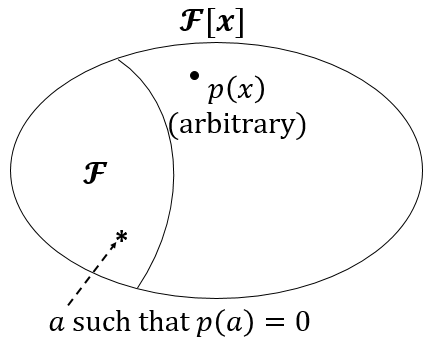
\includegraphics[scale=0.35]{images/algebraically_closed.png}
\caption{$F$ is algebraically closed: every $p(x)\in F[x]$ has an $a\in F$ such  $p(a)=0$.}\label{algebraicallyclosed}
\end{center}
\end{figure}

With this new definition in mind, we can restate Proposition~\ref{proposition:poly:FTOAhard} as follows: 

\begin{prop}{complexalgclosed}
$\mathbb{C}$ is algebraically closed.
\end{prop}

There are fields  besides $\mathbb{C}$ that are algebraically closed,  but there are  also  lots of fields that aren't:

\begin{exercise}{}
\begin {enumerate}[(a)]
\item
Are the rational numbers algebraically closed? Justify your answer.
\item
Are the real numbers algebraically closed? Justify your answer.
\end{enumerate}
\end{exercise}

\begin{exercise}{}
\begin{enumerate}[(a)]
\item
In the field $\mathbb{Z}_5$, evaluate the polynomial $x^4+2$  for all elements of  $\mathbb{Z}_5$.
\item
Using part (a), show  that $\mathbb{Z}_5$ is not algebraically closed.
\item
Use the polynomial $x^6 + 2$ to determine whether or not $\mathbb{Z}_7$ is algebraically closed.
\end{enumerate}
\end{exercise}

In Section~\ref{subsec:FTOAhard} we proved polynomial factorization (Proposition~\ref{proposition:poly:complexlinear}), namely that any polynomial in $\mathbb{C}[x]$ factors as a product of linear factors. The very same proof goes through for any algebraically closed field $F$.  Thus we have:

\begin{prop}{algClosedLinear}
Let $F$ be an algebraically closed field. Then any polynomial $p(x)$  of degree $n$ in $F[x]$ can be completely factored as a constant times a product of $n$ linear terms,   as follows:
\begin{equation}
p(x) = b(x -a_1)(x-a_2) \ldots (x - a_n),
\end{equation}
where $b,a_1,\ldots,a_n \in F$.
\end{prop}



\subsection{Field extensions and algebraic elements}
We've seen quite a few fields that are not algebraically closed. For example, the rational numbers $\mathbb{Q}$ are not algebraically closed, because e.g. $x^2 - 2$ has no  roots in $\mathbb{Q}$.  However, we were able to find a larger field (namely $\mathbb{R}$) that contains $\mathbb{Q}$ which has the root that $\mathbb{Q}$ is lacking. In this section, we'll talk about situations like this in a general context. 


First we need some  terminology to describe the case where one field is contained in  another:


\begin{defn}\label{def:subfield}  
Given a field $E$ and $F\subset E$, then $F$ is called a \term{subfield} of $E$ if $F$ is also a field with the same field operations as $E$. Conversely, $E$ is called an \term{extension field}\index{Field!extension} of $F$.
 \end{defn}

The following exercise should  bolster your understanding of Definition~\ref{def:subfield}

\begin{exercise}{}
\begin{enumerate}[(a)]
\item
Give an example of a field $F$ that has a nontrivial extension field (that is, the extension field contains elements that are not in $F$).
\item
Give an example of a field, $F$ that is a subset of a field $E$, but is not a subfield of $E$. Explain.
\end{enumerate}
\end{exercise}

%\begin{solution}{}
%\begin{enumerate}[(a)]
%\item
%We know that $R\subset C$ and they have the same field operations. Therefore $R$ is a subfield of $C$ and $C$ is an extension field of $R$. The field extension is written as $C/R$.
%\item
%Consider the field, $Z_n\subset R$. The two fields do not have the same field operations, therefore $R/Z_n$ is not a field extension.
%\end{enumerate}
%\end{solution}

We also need terminology to describe roots of polynomials in $F[x]$ that aren't in $F$:

\begin{defn}\label{def:algover}  
Let $F$ be a subfield of $E$, and let $a\in E$. If $p(a)=0$ for some $p(x) \in F[x]$, then $a$ is \term*{algebraic}\index{Algebraic!element, of a field}\index{Field!algebraic element of} over $F$ (see Figure \ref{algebraicelement}). Otherwise, $a$  is \term*{transcendental}\index{Transcendental!element, of a field}\index{Field!transcendental element of} over $F$.
\end{defn}

\begin{figure}
\begin{center}
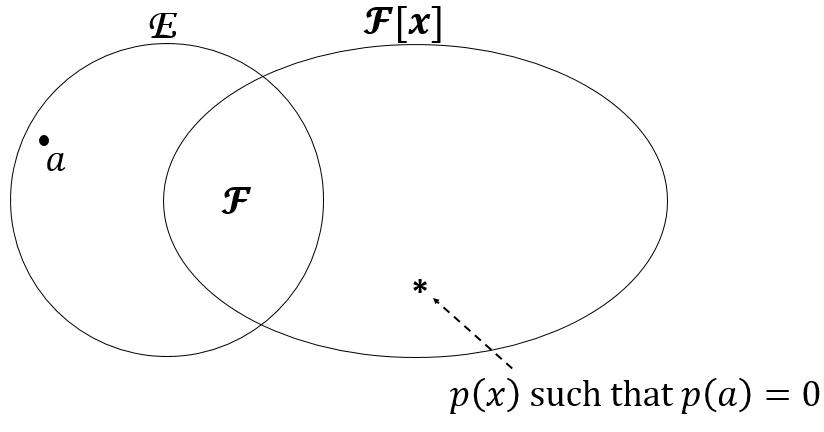
\includegraphics[scale=0.35]{images/algebraic_element.png}
\caption{$a\in E$ is algebraic over $F$:  there exists $p(x)\in F[x]$ such that $p(a)=0$.}\label{algebraicelement}
\end{center}
\end{figure}

\begin{exercise}{}
\begin {enumerate}[(a)]
\item
Give an example of a complex number $z \in \mathbb{C}\setminus \mathbb{R}$ which is algebraic over $\mathbb{Q}$ (in other words, $z$ satisfies $f(z)=0$ where $f(x) \in \mathbb Q[x]$). Justify your answer.
\item
Suppose that $z \in \mathbb{C}$ is algebraic over $\mathbb{R}$. Show that $\bar{z}$ is also algebraic over $\mathbb{R}$.
\item
Show that every element of $\mathbb{C}$ is algebraic over $\mathbb{R}$.
\end{enumerate}
\end{exercise}


\begin{exercise}{}
\begin {enumerate}[(a)]
\item
Given that $a \in \mathbb{C}$ is algebraic over $\mathbb{Q}$, show that $\sqrt{a}$ is also algebraic over $\mathbb{Q}$.
\item
Given that $a \in \mathbb{C}$ is algebraic over $\mathbb{Q}$, show that $a^{1/n}$ is also algebraic over $\mathbb{Q}$ for any natural number $n$.
\end{enumerate}
\end{exercise}


\begin{rem}\label{remark:poly:transcendental}
It's not so easy to show that elements are transcendental. This is because to show that $a$ is transcendental over $F$, you need to show that there's no polynomial whatsoever in $F[x]$  which has $a$ as a root. Let's consider in particular the case $F = \mathbb{Q}$. We saw in Chapter~\ref{complex} that $\mathbb{R}$ has lots of \emph{irrational} numbers, but so far we haven't definitely identified any real number that is transcendental over $\mathbb{Q}$. 

In 1844, Joseph Liouville gave the first proof that a transcendental number exists.  Liouville constructed a number (using infinite series) with special properties, and was able to show that it's impossible to construct a polynomial in $\mathbb{Q}[x]$ that has that number as a root. Hermite showed about 30 years later that $e$ was transcendental, and $\pi$ was added to the list (by Lindemann) 10 years after that. 

Even today, only  a handful of classes of numbers have been shown to be transcendental. This is not to say that there aren't lots of them. In fact, Georg Cantor in 1874 was able to show that ``almost all'' real numbers are transcendental over $\mathbb{Q}$. This is a fascinating topic, and there's lots of information on the Internet if you're interested in pursuing it further (one place to look is 
\url{http://mathworld.wolfram.com/TranscendentalNumber.html}).
\end{rem}

%\begin{solution}{}
%\begin {enumerate}[(a)]
%\item
%Consider $p(x)=x^2+3$. We see that $p(x)\in \mathbb{R}[x]$, because its coefficients are real. But the roots of $p(x)$ are $\pm \sqrt3 i$, which are not real. Also $R \subset C$ and they have the same field operations. Therefore, $\sqrt3 i$ and $-\sqrt{3}i$ are both algebraic over $R$.
%\item
%Consider the natural number $e\in R/Q$; which is not the root of any polynomial in $\mathbb{Q}[x]$. Also $Q\in R$ and they have the same field operations. Therefore, $e$ is transcendental over $R$.
%\item
%Consider $\pi\in C/Q$; which is not the root of any polynomial in $\mathbb{Q}[x]$. Also $Q\in R$ and they have the same field operations. Therefore, $\pi$ is transcendental over $Q$. Now let $p(x)=x-\pi\in \mathbb{R}[x]$. This shows that $\pi$ is the root of a polynomial in $\mathbb{R}[x]$ Therefore, $\pi$ is algebraic over $R$.
%\end{enumerate}
%\end{solution}

For field extensions which have no transcendental elements, the following definition applies:

\begin{defn}\label{def:algfieldextension}  
Suppose $E$ is an extension field of $F$. Then $E$ is called an \term{algebraic extension}\index{Field!algebraic extension} of $F$ if every $a\in E$ is algebraic over $F$. %Otherwise, $E$ is transcendental if it contains at least one $a$ such that $a$ is transcendental over $F$. 
%$E$ is called a \term{transcendental extension} of $F$.
 \end{defn}

\begin{exercise}{}
\begin{enumerate}[(a)]
\item
Give an example of a extension field that is algebraic. Justify your answer.
\item
Give an example of a field extension that is not algebraic. Justify your answer.
\end{enumerate}
\end{exercise}

A field extension may be algebraic, but still contain polynomials that have no roots. There's a special term for field extensions which contain roots for \emph{all} their polynomials:

%\begin{solution}{}
%\begin{enumerate}[(a)]
%\item
%Consider the field extension $C/R$. Every $a\in C$ can be shown to be a root of some polynomial in $\mathbb{R}[x]$. Therefore, every $a\in C$ is algebraic over $R$ and we say that $C/R$ is an algebraic field extension.
%\item
%Consider the field extension $R/Q$. We know that $\pi\in R$, but it can be shown that $\pi$ is not the root of any polynomail in $\mathbb{Q}[x]$. Therefore, $\pi$ is transcendental over $Q$ and we say that $R/Q$ is a transcendental field extension.
%\end{enumerate}
%\end{solution}

\begin{defn}\label{def:algclosure}  
Let $E$ be an algebraic extension field of $F$. Suppose that for every $p(x) \in E[x]$, there exists $a \in E$ such that $p(a)=0$.  Then  $E$ is  an \term*{algebraic closure}\index{Field!algebraic closure of}\index{Algebraic closure!of a field} of $F$ (see Figure \ref{algebraicclosure}).
\end{defn}

\begin{figure}
\begin{center}
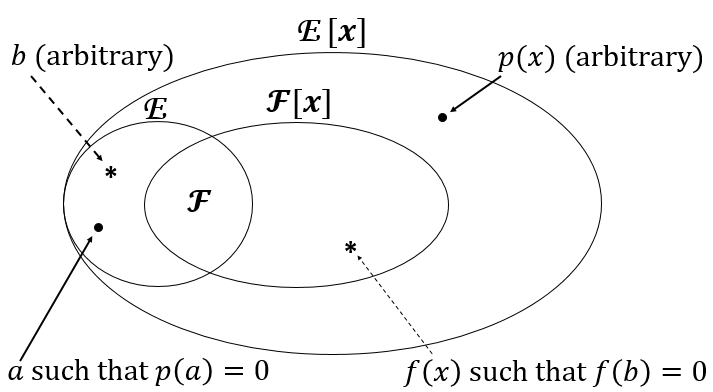
\includegraphics[scale=0.35]{images/algebraic_closure.png}
\caption{$E$ is an algebraic closure of $F$:  every $p(x)\in E[x]$ has an $a\in E$ such that $p(a)=0$; and every $b\in E$ has an $f(x)\in F[x]$ such that $f(b)=0$.}\label{algebraicclosure}
\end{center}
\end{figure}

Here's an example of an algebraic closure:

\begin{prop}{realalgclosure}
$\mathbb{C}$ is an algebraic closure of $\mathbb{R}$.
\end{prop}


\begin{proof}{}
Let $a+bi \in \mathbb{C}$ be arbitrary and let $p(x)=(x-(a+bi))(x-(a-bi))= x^2-2ax+a^2+b^2\in\mathbb{R}[x]$. We see that $a+bi$ is a root of $p(x)$. Since $a+bi$ is arbitrary, we can say that any element of $\mathbb{C}$ is a root of some polynomial in $\in\mathbb{R}[x]$. By Definition~\ref{def:algfieldextension} this makes $\mathbb{C}$ an algebraic extension of $\mathbb{R}$. Additionally, by Proposition~\ref{proposition:rings:complexalgclosed}, $\mathbb{C}$ is algebraically closed. Therefore, by Definition~\ref{def:algclosure}, $\mathbb{C}$ is the algebraic closure of $\mathbb{R}$.
\end{proof}

Does every field have an algebraic closure? Let's look at some field extensions we're already familiar with:

\begin{exercise}{}
\begin{enumerate}[(a)]
\item
Give an example that shows that $\mathbb{C}$ is not an algebraic closure of $\mathbb{Q}$ . Explain.
\item
Give an example that shows that $\mathbb{R}$ is not an algebraic closure of $\mathbb{Q}$ . Explain.
\end{enumerate}
\end{exercise}


Although we won't prove it here, it can be shown that every field has an algebraic closure.
\footnote{see  \url{https://soffer801.wordpress.com/2011/10/25/every-field-has-an-algebraic-closure/} for a nice discussion.} In particular, there is a subfield of $\mathbb{C}$ which is an algebraic closure of $\mathbb{Q}$: this subfield is called the field of \term{algebraic numbers}.

\begin{exercise}{}
Draw a set diagram that shows the relationships between the sets $\mathbb{Q}, \mathbb{R}, \mathbb{C}$, and $\mathbb{A}$, where $\mathbb{A}$ denotes the set of algebraic numbers.  (For example, the ``set bubble'' representing $\mathbb{Q}$ should be inside the bubble representing $\mathbb{C}$, since $\mathbb{Q} \subset \mathbb{C}$.)
\end{exercise}

\subsection{Applications of algebraic field extensions}

We've already seen how field extensions play an important role in mathematics.  The irrational numbers were first introduced using an algebraic  field extension  of $\mathbb{Q}$  (although later it was discovered that not all irrational numbers are algebraic over $\mathbb{Q}$).  Similarly, the complex numbers were created as an algebraic field extension of the real numbers.  But this is just the beginning. Algebraic field extensions have played a pivotal role in a great number of deep mathematical results obtained over the last 200 years. Here is a short list of results which make use of algebraic field extensions:

\begin{itemize}
\item 
The quadratic formula expresses the roots of quadratic polynomials  in terms of algebraic operations on the coefficients plus a square root. There are similar (but vastly more complicated) formulas for solving cubic and quartic (3rd and 4th degree)  polynomial equations, which involve algebraic operations and  taking $n$th roots, for different values of $n$.  How about quintic (5th degree) polynomials?  Amazingly, it is possible to prove that there is no general formula for the solution of a quintic equation in terms of roots and algebraic operations.  Not just the formula is not known--there is \emph{no formula}. Period. This stupendous result is associated with the mathematicians Evariste Galois, Niels Henrik Abel, and Paolo Ruffini, and was proved in the mid-19th century.

This result relates to field extensions because every solution to an equation that involves only roots and algebraic operations must belong to certain type of field extension of the rationals. This fact imposes conditions on the type of numbers that can be expressed in such a form. It can be shown that there are roots of 5th-degree equations that don't meet these conditions---hence they can't possibly satisfy such an equation.

\item
Beginning with the Greeks,  mathematicians tried for thousands of years to find a way to trisect an angle, using only straightedge and compass. In 1837, Pierre Wantzel finally showed that it is \emph{impossible}. His proof built on previous results of Galois. (Think of how many hours over how many centuries were spent on a futile quest!)

This result relates to field extensions in similar fashion as the previous one. Geometrical points in the plane are identified as complex numbers (as we described in Section~\ref{complex_roots}). Every point constructed based on a set of  points is an algebraic combination of the corresponding complex numbers, together with square roots. This means that every constructable point must be contained in a series of field extensions created by successively adding square roots to an existing field. It can be shown that trisecting an angle involves finding a cube root which cannot possibly belong to such a series of extensions.  You may consult:

\noindent
 \footnotesize{\url{https://terrytao.wordpress.com/2011/08/10/a-geometric-proof-of-the-}}\\
 \footnotesize{\url{impossibility-of-angle-trisection-by-straightedge-and-compass/}}

\noindent
 to get a flavor of how this proof goes.
\item
A similar constructability problem is known as ``squaring the circle'':  Given a square of side 1, find a circle with the same area using only straightedge and compass. This can be shown to be impossible, as a consequence of the transcendence of $\pi$ alluded to in Remark~\ref{remark:poly:transcendental}.
\end{itemize}

\section{References}
\label{sec:rings:refs}

The following links talk about different applications of rings:

\noindent \url{https://pdfs.semanticscholar.org/8ff4/9f31c24cc10b72af379fa364becc89eb5a36.pdf}

\noindent \url{https://wdjoyner.files.wordpress.com/2018/04/sm462-notes-on-ring-thry.pdf}

\noindent \url{http://www.ihes.fr/~brown/GergenLectureI.pdf}

\noindent \url{https://www.wireilla.com/ns/maths/Papers/3414ijscmc05.pdf}

\noindent \url{http://math.mit.edu/~mckernan/Teaching/12-13/Spring/18.703/book.pdf}

\noindent \url{https://www.math.ias.edu/~avi/PUBLICATIONS/HrubesWi2013.pdf}

\noindent \url{http://ijgt.ui.ac.ir/article_5453_9f9342e7224465dd42f3537a6a7fe39a.pdf}



% Applications of field extensions
% Field extensions and solvability of polynomial equations by radicals
% Give example of quadratic formula. There is a formula for cubic and quartic.  There is no formula for quintic. Not just the formula is not known--there is NO FORMULA. Proving this has to rank as one of the great intellectual achievements of all time.
% In this section, give you some idea of the methods involved in this proof.
% Show adding sqrt gives extension field.
% Consider quadratic formula. Shows that  the root is in extension field
% Add other square roots. produces another field extension.
% Transcendental over 


% Impossible constructions using straightedge and compass.
% Every complex number constructed based on a set of points  is the root of a quadratic equation 
% The set of all constructable points is contained in a field extension obtained by adding successive square roots.  This limits the types of numbers that can be constructed.
% Extension using square roots.  Can show that there are cube roots which are not in any field extension obtained in this manner.
%https://terrytao.wordpress.com/2011/08/10/a-geometric-proof-of-the-impossibility-of-angle-trisection-by-straightedge-and-compass/
% Squaring the circle. Amounts to constructing $\sqrt{\pi}$. If this is possible, then 
% Prove that if \sqrt{pi} is algebraic, then \pi is also algebraic.


%Now that we understand what it means for an element to be algebraic over or transcendental over a field, we can further our discussion into extension fields.  The theory of extension fields has played a critical role in the development of mathematics. For example, the ancient Greeks used geometry to construct rational numbers from line segments, but could not construct the square root of prime numbers, which they encountered  as hypotenuses of some right triangles.
% Irrational square roots give extension fields for the rational numbers
%$ a + b\sqrt{2}$ is an extension field of rationals
%real are extension field of rationals
%Before we go on with our discussion though, we must consider a couple of definitions.


%\begin{solution}
%Consider $\pi$. We know that $\pi\in C$, but it can be shown that $\pi$ is not the root of any polynomail in $\mathbb{Q}[x]$. Therefore, $C$ is not the algebraic closure of $Q$.
%\end{solution}

% Say something about extension fields
% The theory of extension fields has played a critical role in the development of mathematics. 
% Irrational square roots give extension fields for the rational numbers
% a + b\sqrt{2} is an extension field of rationals
%real are extension field of rationals
%e, pi, irrational that dont have
%if a set has no proper field extensions, then it is algebraically closed

%
%
%\section{Irreducible Polynomials}
% 
% 
%A nonconstant polynomial $f(x) \in F[x]$ is \term{
%irreducible}\index{Polynomial!irreducible}\index{Irreducible polynomial}
%over a field $F$ if $f(x)$ cannot be expressed as a product of two
%polynomials $g(x)$ and $h(x)$ in $F[x]$, where the degrees of $g(x)$
%and $h(x)$ are both smaller than the degree of $f(x)$.  Irreducible
%polynomials function as the ``prime numbers'' of polynomial rings.
% 
% 
%\begin{example}{poly_irred}
%The polynomial $x^2 - 2 \in {\mathbb Q}[x]$ is irreducible since it
%cannot be factored any further over the rational numbers. Similarly,
%$x^2 + 1$ is  irreducible over the real numbers. 
%\end{example}
% 
% 
%\begin{example}{finite_poly}
%The polynomial $p(x) = x^3 + x^2 + 2$ is irreducible over ${\mathbb
%Z}_3[x]$. Suppose that this polynomial was reducible over ${\mathbb
%Z}_3[x]$.  By the division algorithm there would have to be a factor
%of the form $x - a$, where $a$ is some element in ${\mathbb Z}_3[x]$.
%Hence, it would have to be true that $p(a) = 0$.  However,
%\begin{align*}
%p(0) & = 2 \\
%p(1) & = 1 \\
%p(2) & = 2.
%\end{align*}
%Therefore, $p(x)$ has no zeros in ${\mathbb Z}_3$ and must be
%irreducible. 
%\end{example}
%
%
%\begin{lemma}\label{poly:integer_coef_lemma}
%Let $p(x) \in {\mathbb Q}[x]$.  Then
%\[
%p(x) = \frac{r}{s}(a_0 + a_1 x + \cdots + a_n x^n),
%\]
%where $r, s, a_0, \ldots, a_n$ are integers, the $a_i$'s are
%relatively prime, and $r$ and $s$ are relatively prime. 
%\end{lemma}
% 
% 
%\begin{proof}
%Suppose that
%\[
%p(x) = \frac{b_0}{c_0} + \frac{b_1}{c_1} x + \cdots + \frac{b_n}{c_n}
%x^n,
%\]
%where the $b_i$'s and the $c_i$'s are integers. We can rewrite $p(x)$
%as 
%\[
%p(x) = \frac{1}{c_0 \cdots c_n} (d_0 + d_1 x + \cdots + d_n x^n),
%\]
%where $d_0, \ldots, d_n$ are integers. Let $d$ be the greatest common
%divisor of $d_0, \ldots, d_n$.  Then
%\[
%p(x) = \frac{d}{c_0 \cdots c_n} (a_0 + a_1 x + \cdots + a_n x^n),
%\]
%where $d_i = d a_i$ and the $a_i$'s are relatively prime. Reducing $d
%/(c_0 \cdots c_n)$ to its lowest terms, we can write
%\[
%p(x) = \frac{r}{s}(a_0 + a_1 x + \cdots + a_n x^n), 
%\]
%where $\gcd(r,s) = 1$.
%\end{proof}

